% ------------------------------------------------------------------------
% ------------------------------------------------------------------------
% abnTeX2: Modelo de Trabalho Acadêmico (tese de doutorado, dissertação de
% mestrado e trabalhos monográficos em geral) em conformidade com
% as normas da ABNT
% ------------------------------------------------------------------------
% ------------------------------------------------------------------------

\documentclass[english, 
               brazil, 
               msc] %Opções msc (Mestrado)
               {ppgpi-abntex2}
% Geração de dummy text
% Retirar para a versão final do documento


%Compila o indíce
\makeindex

\begin{document}

% Seleciona o idioma do documento (conforme pacotes do babel)
\selectlanguage{brazil}

% Retira espaço extra obsoleto entre as frases.
\frenchspacing 

% ----------------------------------------------------------
% ELEMENTOS PRÉ-TEXTUAIS
% ----------------------------------------------------------

\pretextual


\titulo{Empreendedorismo e Competências Empreendedoras: Programa Empreenda Agro Sustentável como mecanismo indutor para geração de inovação}
\orientador{Prof. Dr. Francisco Sandro Rodrigues Holanda}
\author{Luiz Diego Vidal Santos}


\curso{Ciência da Propriedade Intelectual}

\imprimircapa

\imprimirfolhaderosto

%\imprimirfichacatalografica
%\imprimirfolhadeaprovacao
%\begin{dedicatoria}
   \vspace*{\fill}
   \centering
   \noindent
   \textit{Dedico essa dissertação aos meus pais, verdadeiramente os grandes mestres que empenharam amor e suor na formação dos seus filhos.} \vspace*{\fill}
\end{dedicatoria}
% ---
%\begin{agradecimentos}

A minha família pelo apoio, colaboração, amor, empenho e paciência. 

A minha noiva pelo apoio nos momentos difíceis e de vontade de desistência, me guiando para o melhor caminho.

Ao meu orientador pela oportunidade de me expressar inventivamente, me apoiar durante todo o projeto assim como orientar nos desvarios que surgiram no meio do caminho.

As Empresas que apoiaram no desenvolvimento deste projeto: SEBREA, CREA-SE,AEASE, Agroconsulte, IP Sustentabilidade, IMAZON.

Ao Centro de Ciências agrárias e Aplicadas pela permissão e apoio no desenvolvimento do Programa

Aos colegas de curso pela amizade, companheirismo, espontaneidade e alegria ao longo desses anos de convivência.

E, finalmente, a Deus pela fé e força depositadas em mim para que eu pudesse enfrentar este curso e conseguir concluí-lo.
\end{agradecimentos}
% ---
%\begin{epigrafe}[]
    \vspace*{\fill}
	\begin{flushright}
	
		\textit{"A plenitude da atividade humana é alcançada somente quando nela coincidem, se acumulam,\\ se exaltam e se mesclam o trabalho o estudo e o jogo; isto é,  quando nós \\ trabalhamos, aprendemos e nos divertimos, tudo ao mesmo tempo."\\
				\textbf{Domenico de Masi}}
		
	\end{flushright}
\end{epigrafe}
% ---
% resumo em português
\setlength{\absparsep}{18pt} % ajusta o espaçamento dos parágrafos do resumo
\begin{resumo}

Ser empreendedor não significa apenas ter seu próprio negócio, o empreendedorismo está ligado às ações e capacidades individuais, ou seja, possuir características empreendedoras é ser capaz de criar, modular e sustentar ideias inovadoras globalmente, assim as ideias normalmente estão ligadas à inovação algo que transcende o comum. Algumas ferramentas tais como workshops, jornadas, cursos, palestras podem ser usadas para difusão do comportamento empreendedor tanto em órgãos privados como em instituições de ensino, ou seja, incutir novas ações empreendedoras no sentido comercial, nas áreas industriais e agrícolas que sejam sustentáveis. Faz-se necessário, então, a construção de um cenário favorável ao desenvolvimento da cultura empreendedora no ambiente acadêmico, principalmente nas ciências agrárias. Para construção deste senário, muitas nações estão buscando promover a atividade empreendedora, utilizando para isto programa educacionais promovidos nos meios acadêmicos alcançando um importante público os jovens. Assim, torna-se evidente que o sistema educacional que promova o desenvolvimento das competências empreendedoras tem um importante papel a cumprir para com a causa empreendedora. Neste sentido, este estudo estudo tem como objetivo, identificar de forma analítica a inovação sustentável e a eficácia da promoção empreendedora por meio de uma ação de educação com vistas aos negócios rurais, tendo como ferramenta promotora o Programa Empreenda Agro Sustentável. O Programa visa buscar o engajamento dos alunos para o desenvolvimento de novos negócios direcionados ao setor agrícola, podendo este experimento também direcionar futuras pesquisas científicas focadas em produtos capazes de satisfazer às novas demandas, de forma eficiente e sustentável. A metodologia de natureza quantitativa exploratória e de estudo de caso, foi utilizada para avaliar quantitativamente o Programa Empreenda AGRO Sustentável, com análise dos dados, que foram coletados por meio da técnica quantitativa “survey” tendo como base o estudo GUESS. A ferramenta de promoção prática do exercício do comportamento empreendedor “Programa Empreenda AGRO Sustentável", foi conduzida buscando a disseminação do empreendedorismo junto aos acadêmicos do Centro de Ciências Agrárias Aplicadas da Universidade Federal de Sergipe – UFS. Foram conduzidos quatro Workshops, planejados de forma sistemática e interativa, sendo aplicadas ferramentas para modelagem de negócios como Design Thinking visando despertar ideias de startups em oficinas interdisciplinares fomentando desta forma a construção de Mínimos Produtos Comercialmente Viáveis (MCVP). Por meio do Programa Empreenda Agro Sustentável e a partir da aplicação das metodologias ativas, 15 equipes discutiram e amadureceram ideias em modelos de startups, resultando em modelos de negócios escaláveis e negociáveis direcionados ao meio rural. Pode-se perceber também que os alunos participantes apresentam forte influência positiva na intenção empreendedora e na autoeficácia para o empreendedorismo. Por meio dos resultados obtidos nesta pesquisa ficou evidente que, os alunos envolvidos no decorrer do programa evoluíram positivamente as dimensões empreendedoras estudadas, influenciando assim o desenvolvimento de novos negócios planejados na etapa de pré-aceleração, e encontram maior segurança para o próximo passo que é o de aceleração de seus planos de negócios, conquistando autonomia, buscando novas oportunidades, como profissionais proativos com destaque no mercado de trabalho.

\textbf{Palavras-chave}: Empreendedorismo; Competências empreendedoras; Negócios sustentáveis; Propriedade Intelectual; Projeto de Extensão.
\end{resumo}


% resumo em inglês
\setlength{\absparsep}{18pt} % ajusta o espaçamento dos parágrafos do resumo
\begin{resumo}[Abstract]
 \begin{otherlanguage*}{english}
   
Being an entrepreneur does not just mean having your own business, entrepreneurship is linked to individual actions and capabilities to create, modulate and sustain innovative ideas globally. Thus, ideas are usually linked to innovation, something that transcends the ordinary. Some tools such as workshops, seminars, courses, lectures can be used to disseminate entrepreneurial behavior both in private bodies and in educational institutions, in order to instill new sustainable entrepreneurial actions, in the commercial sense, in the industrial and agricultural areas in the academic environment. . It is necessary, then, to build a favorable scenario for the development of entrepreneurial culture in the academic environment, mainly in the agricultural sciences. In this context, many nations are seeking to promote entrepreneurial activities, using educational programs promoted in academic circles to reach an important young audience. In this sense, this study aims to identify, in an analytical way, sustainable innovation and the effectiveness of encouraging entrepreneurship through an educational action aimed at rural businesses, using the Empreenda AGRO Sustentável Program as a promoting tool. The Program aims to seek student engagement for the development of new businesses aimed at the agricultural sector, and this experiment can also direct future scientific research focused on products capable of satisfying new demands, in an efficient and sustainable manner. The methodology of quantitative exploratory nature and case study was used to quantitatively evaluate the Empreenda AGRO Sustentável Program with data collection using the “survey” technique based on the GUESS study. The tool for the practical promotion of entrepreneurial behavior “Programa Empreenda AGRO Sustentável” was conducted seeking the dissemination of entrepreneurship among academics at the Center for Applied Agricultural Sciences at the Federal University of Sergipe (UFS). Four workshops were planned and executed in a systematic and interactive way , in which methodologies and tools for business modeling such as Design Thinking were applied in order to awaken ideas from startups through interdisciplinary workshops, thus promoting the construction of Minimum Commercially Viable Products (MCVP). Sustainable and based on the application of active methodologies, 15 teams discussed and matured ideas in models of startups, resulting in scalable and negotiable business models aimed at the rural environment. As a result, the research found that the participating students had a strong positive influence on the intention entrepreneur a and self-efficacy for entrepreneurship. In addition, the research demonstrated that the students involved in the course of the program positively evolved the entrepreneurial dimensions studied, thus influencing the development of new businesses planned in the pre-acceleration stage, and found greater security for the next step, which is the acceleration of their business plans, gaining autonomy, seeking new opportunities as proactive professionals in the job market.

 \textbf{Keywords}:Sustainable business, Intellectual Property, Extension Project.
 \end{otherlanguage*}
\end{resumo}
    
 %Lista de Figuras %%%%%%%%%%%%%%
    \pdfbookmark[0]{\listfigurename}{lof}
     \listoffigures*
   \cleardoublepage

% Lista de Tabelas %%%%%%%%%%%%%
    \pdfbookmark[0]{\listtablename}{lot}
     \listoftables*
    \cleardoublepage

\cleardoublepage
   
% ---
% inserir lista de abreviaturas e siglas
% ---

\begin{siglas}
    
  	\item[EE]{Educação Empreendedora}
  	%\item[DB]{Data Base}
  	\item[INPI]{Instituto Nacional da Propriedade Intelectual}
  	\item[PI]{Propriedade Intelectual}
  	\item[GUESSS]{\textit{Global University Entrepreneurial Spirit Students Survey}}
  	\item[EAESP]{Escola de Administração de Empresas de São Paulo}
  	\item[FGV]{Fundação Getúlio Vargas}
  	\item[ABP]{ Aprendizagem Baseada em Problemas}

\end{siglas}
% ---
%% ---
% inserir lista de símbolos
% ---

\begin{simbolos}
  \item[$ \sum  $] Letra grega Sigma
  \item[$ \int $] Integral
  \item[$ \omega $] Letra grega ómega
\end{simbolos}
% ---
\pdfbookmark[0]{\contentsname}{toc}
\tableofcontents*
\cleardoublepage

% ----------------------------------------------------------
% ELEMENTOS TEXTUAIS
% ----------------------------------------------------------
\textual
\chapter{INTRODUÇÃO}

\section{JUSTIFICATIVA}

Sabe-se que o campo de trabalho para os novos dos profissionais atuantes na área das ciências agrárias tem mudado, a busca pela valorização das capacidades e competências profissionais. Busca-se cada vez mais a afirmação e promoção de direitos de cidadania, associatividade política, responsabilidade social e ambiental, consideração, respeito as diversidades étnicas e culturais que devem ser valorizadas constantemente, para tal, a academia  tem um papel importante neste contexto, que é  o de fomentar e oportunizar essas competências. Dentro deste contexto a capacidade de manter-se fio a inovação, especialmente a destrutiva é fundamental ao progresso do crescimento e manutenção futura do profissional das agrárias no novo mercado de trabalho, assim como saber lidar com os novos empreendimentos nos campos de atuação.

De acordo com \citeonline{tarapanoff_monitoramento_2016}, existe um cenário favorável para os negócios rurais que buscam a sustentabilidade econômica e ambiental. Nesse sentido o Brasil deve buscar trilhar  um caminho seguro em relação à sustentabilidade de seu agronegócio, em consonância com as melhores práticas da exploração ambiental e a produção agrícola, parte promovida por cumprimentos a regras ambientais a exemplo a Agenda 2030 que prevê a exploração consciente dos recursos naturais e tomando medidas urgentes sobre a mudança climática individuais quanto institucionais, \cite{filho_documentos_2017}.

O desenvolvimento sustentável pode ser definido segundo \cite{lara_ideologia_2017} como um negócio socialmente responsável e ecologicamente correto, mas invariavelmente viável em termos financeiros. Concomitantemente existe uma lacuna na formação profissional durante o ensino superior no que se refere à adoção de uma cultura empreendedora, \cite{lima_ser_2015}. Não tem sido possibilitado aos acadêmicos, a oportunidade de gerar inovação tecnológica sustentável, inclusive como forma de aplicação prática dos conhecimentos adquiridos. Da mesma maneira, é sabido que para uma ideia inovadora alcançar o sucesso desejado é preciso muito mais que o conhecimento técnico. É necessário que seja disponibilizado aos futuros profissionais/empreendedores treinamento na formulação das ideias em etapas direcionadas e adequadamente orientadas.

Para que um negócio sustentável possa ter sucesso é preciso mais do que uma ideia inovadora, deve ter o meio e os profissionais capacitados para tal, Relatórios da Fundação Kauffman afirma que as Startups criam uma média de 3 milhões de novas vagas de empregos anualmente e que, estes tipos de empreendimentos serão responsáveis pela criação de mais de 50\% dos empregos no  mundo  \cite{brasil_o_2017}. Atualmente estes tipos de  negócios contribuem para o crescimento de diversas regiões geográficas, já que não se expandem apenas em tamanho, mas também em novos locais, além de incentivar o emprego em suas indústrias relacionadas. Supletivamente, como muitas dessas microempresas são responsáveis por desenvolver novas tecnologias e processos, elas também geram aumento de absorção do capital humano mais capacitado para gestão e gerência.

Diante deste cenário, para que o aprendizado dos profissionais seja mais efetivo, surgem diversas abordagens e metodologias a serem assimiladas. Nesse contexto, deve existir uma maior produção de estudos e conteúdos sobre a educação empreendedora e os modelos educacionais que melhor se apliquem ao aprendizado deste, como ressalta \citeonline{kuratako_entrepreneurship_2003}. É notória a urgência de se pesquisar o ensino em empreendedorismo de forma disciplinada no meio acadêmico. Por ser um tema de grande importância, a educação empreendedora promovida no seio da educação superior pode ser o caminho para o surgimento de inovações sustentáveis e economicamente viáveis passives e escaláveis.

Dentro do contexto metodológico educacional, temos as metodologias ativas, que trazem a possibilidade de mudança da centralidade no docente (ensino) para o estudante (aprendizagem), ponto de vista preconizado por \citeonline{freire_pedagogia_1987} ao abordar educação como um processo que não é realizado por outrem, ou pelo próprio indivíduo, mas que acontece na interação entre pessoas através de sua vivência por meio de palavras, ações e reflexões. Enquanto o método tradicional de ensino utiliza a transmissão de informações e concentra as atividades no docente, no método ativo, os alunos ocupam a centralidade da educação e o conhecimento é construído de forma colaborativa. Sucintamente, as metodologias ativas propõem transformar o processo de ensino e aprendizagem na busca pelo comportamento empreendedor, como uma forma de enfrentar o modelo tradicional praticado e aceito ao longo dos anos.
 
As práticas ativas estimulam o reconhecimento dos problemas do mundo atual, tornando os alunos aptos a intervir na promoção das transformações necessárias a exemplo as que se baseiam  na reflexão e argumentação \cite{bezanilla_methodologies_2019}. Assim, o aluno torna-se protagonista da sua aprendizagem e autônomo no alcance dos seus objetivos incorporando seus valores e razões \cite{rubel_student_2016}. Existem vários recursos, ferramentas e estratégias para alcançar o satisfatório comportamento empreendedor, como: uso de tecnologias digitais e aplicativos \cite{pereira_use_2020}, ensino híbrido e suas estratégias como sala de aula em rotação por estações, Aprendizagem Baseada em Problemas (ABP) \cite{souza_aprendizagem_2015}, e uso de situações-problema e estudos de caso, sala de aula invertida \cite{junior_sala_2016,branco_sala_2016}, uso de mapas mentais \cite{junior_percepcao_2018}, sala de aula compartilhada \cite{strack_por_2009}, estratégias de Design Thinking \cite{andrews_circular_2015}, Gamificação \cite{ogawa_avaliacao_2016}, projetos de extensão \cite{garcia_contribuicao_2012}, dentre tantos outros recursos do método ativo, os quais podem vir facilitar o entendimento e a compressão dos acadêmicos das Ciências Agrárias no contexto de um mercado de trabalho que se apresenta com um perfil voltado ao empreendedor.

O empreendedorismo é a capacidade de reunir esforços para transformar em realidade uma oportunidade, objetivando a satisfação pessoal do empreendedor e o lucro. Tal conceito define o empreendedorismo como uma prática constante das atividades rotineiras dos educandos. Desde a capacidade de resolução de problemas quanto a idealização de propostas capazes de inovar. Dentro desta dicotomia entre empreendedorismo e educação surge a "Educação Empreendedora", que por meio de práticas e dinâmicas planejadas busca a melhora na promoção do comportamento empreendedor \cite{martins_educacao_2016, morais_empreendedorismo_2018}, e resolução de problemas de forma sustentável e rápida.

É diante desta problemática que este projeto busca avaliar a inovação sustentável e a eficácia da promoção empreendedora por meio de uma ação de educação com vistas aos negócios rurais, por meio do Programa Empreenda Agro Sustentável promovido para os acadêmicos das ciências agrárias, utilizando para este fim, Workshops encadeados e ferramentas didáticas que buscam capacita-los para a construção de propostas inovadoras viáveis.


\section{DELIMITAÇÕES DO ESTUDO}

Esta pesquisa está focada na dissonância entre a teoria e pratica dos métodos educacionais e as mudanças vertiginosas do mercado de trabalho no meio rural. Este Setor foi escolhido por estar contribuindo significativamente para a balança comercial do país, apresentando saldos positivos frequentes. Da mesma forma contribui para a segurança alimentar do País e produção de produtos limpos e renováveis. O mercado emergente apresenta significativa contribuição para a empregabilidade da população no campo, invertendo cada vez mais o êxodo rural, porém este mercado que absorve novos profissionais, exige que tais profissionais se mostrem a cada dia mais capacitados para lidar com o desenvolvimento tecnológico e a produção em larga escala, em que a busca pela valorização das capacidades e competências profissionais aumenta a cada dia. 

Em contraponto o empreendedorismo atualmente se confunde com a Meritocracia. Tantos a meritocracia quanto o empreendedorismo caminham junto no cerne do movimento de individualização no mundo do trabalho \cite{costa_novo_2019}. Os dois  Projetam imagens individuais de trabalho e sucesso, em que a capacidade individual somada as oportunidades geram resultados positivos junto ao mercado de trabalho. Porém a diferença substancialmente positivos. Porém o Empreendedorismo derivado da educação empreendedora proposto neste projeto, surge atrelado a técnicas e métodos capazes de facilitar e validar as propostas empreendedoras, assim sendo um programa que vise o incentivo as práticas empreendedoras de forma sistemática e coerentes distingue dos resultados negativos que estão atrelados a meritocracia e suas vantagens a frente dos pares distintos.

Visando compreender o comportamento empreendedor nos alunos dos cursos do Centro Ciências Agrárias Aplicadas CCAA da Universidade Federal de Sergipe-UFS, foi escolhida a população para esta pesquisa de 1.453 discentes dos cursos de graduação nas áreas de agrárias da Universidade Federal de Sergipe (UFS): Engenharia Agronômica, Engenharia Agrícola, Zootecnia, Engenharia Florestal, Veterinária e Engenharia de Pesca, dados contidos no relatório estatístico de matriculas 2017 da instituição. A amostra compreenderá  120 discentes que participarem do programa Empreenda Agro Sustentável.

As atividades serão desenvolvidas por meio de quatro Workshops, que constam metodologias ativas, oficinas, palestras com vistas a promover aprendizagem significativa e colaborativa. Durante os módulos do projeto (Workshops), os participantes testarão de seus \textit{insights} para que novas requisições sejam realizadas e/ou que erros nos planejamentos sejam encontrados e, consequentemente, debatidos e mitigados. Depois que todas as Sprints (atividades dos três Workshops) forem finalizadas, ou seja, que todos os módulos sejam abordados, será iniciado um ciclo de Apresentações e desenvolvimento da habilidade de apresentação e demonstração dos produtos por meio apresentações (Pitch). O programa será desenvolvido em quatro encontros (Workshops), que abordarão temas pertencentes ao empreendedorismo e o comportamento empreendedor, a saber: 

\begin{itemize}

\item {1º Workshop: O que é Startups, Empreendedorismo, comportamento empreendedor e cultura empreendedora, Problemas (segmentação do mercado), segundo os Objetivos do Desenvolvimento Sustentável (ODS), Modelagem do negócio e Criatividade;}
\item {2º Workshop: A busca de oportunidades como Característica Empreendedora, Construção do Lean Canvas, Mapa de Empatia, Validação da Proposta de Valor e Economia colaborativa e Coworking; }

\item {3º Workshop: Makeathon: Prototipagem para o MVP, O que você pode fazer por seu cliente e como o cliente adquire seu produto?;}
\item {4º Workshop: Demoday. Destaca-se que o instrumento de pesquisa que será utilizado neste experimento foi composto por Cinco blocos de questões de múltipla escolha baseadas principalmente em escalas de cinco ou sete possibilidades.}
\end{itemize}

O  primeiro conjunto de questões está relacionado a informações que buscam traçar o perfil dos alunos entrevistados, tais como: gênero, faixa etária, curso vinculado e o perfil de interesse nas áreas de estudo ligadas ao empreendedorismo sustentável tal questionário foi baseado no trabalho desenvolvido por \citeonline{lima_ser_2015}. O segundo bloco e composto por 10 questões relacionadas a auto eficácia dos estudantes de múltipla escolha partindo da alternativa “Completamente Inseguro” a "Completamente Seguro”. O terceiro bloco e composto por 7 questões que analisam a intenção empreendedora do aluno da quais segue uma proporção partindo da resposta, tendo como alternativas partido do “Discordo totalmente” a “Concordo totalmente”. O Quarto bloco retrata a intensão ter sua própria empresa ou ser autônomo e por fim o Quinto bloco contendo 11 questões sobre a ligação da família e o apoio familiar no empreendedorismo, tendo como alternativas partido do “Discordo totalmente” a “Concordo totalmente”. Buscando aferir os resultados do programa, um novo questionário abordando as mesmas temáticas será aplicado ao final do programa. 
O estudo caracteriza-se como uma pesquisa de levantamento ou Survey, que se destaca por compreender uma amostra expressiva em relação ao universo pesquisado. Optou-se por adotar a abordagem qualitativa para a análise dos dados quanto a percepção do comportamento empreendedor dos alunos, e a abordagem quantitativa na mensuração dos resultados educacionais do Programa Empreenda Agro Sustentável. Após a aplicação dos instrumentos de análise, será realizada a categorização dos dados para que seja possível a classificação da pontuação segundo o questionário GUESS que utilizada testes de hipóteses sobre uma proporção. O projeto traz como benefícios: 

\begin{itemize}
\item{Promover o desenvolvimento pessoal, econômico e social no meio rural por meio de oportunidade de acesso a alternativas de geração de renda;}
\item{Criar a oportunidade de se trabalhar com o que realmente gosta e vencer os entraves do mercado econômico;}
\item{Dar autonomia e liberdade para conduzir o próprio talento, porem orientado por metodologias especificas;}
\item{Transmitir valores e inspirar novos empreendedores no ambiente agrário;}
\item{Ensinar como lidar com os fracassos e frustrações, sabendo como contorna-los;}
\item{Ensinar estratégias de planejamento de ideias ou carreiras buscando geração de renda;}
\end{itemize}


\section{OBJETIVOS}

\subsection{OBJETIVO}

Avaliar o impacto do Programa Empreenda Agro Sustentável como mecanismo indutor de competência empreendedora com inovação no setor do agronegócio junto aos acadêmicos das Ciências Agrárias da UFS.



\subsection{OBJETIVOS ESPECÍFICOS}

\begin{itemize}
\item{Identificar o efeito da promoção de iniciação empreendedora direcionado a inovação sustentável no meio acadêmico;}
\item {Avaliar o potencial empreendedor dos alunos do Centro de Ciências Agrárias Aplicadas participantes do Programa;
}
\item {Fomentar por meio do projeto de extensão o comportamento empreendedor nos alunos do Centro de Ciências Agrárias Aplicadas;}

\item {Tipificar e analisar os tipos de PI que surgem com o incentivo ao empreendedorismo sustentável por meio da aplicação das metodologias trabalhadas no Programa.}

\end{itemize}


\section{PROBLEMA}

O comportamento empreendedor como indutor de inovação, pode ser estimulado mediante o uso de projetos de extensão universitária como o Programa Empreenda Agro Sustentável? 


\section{HIPÓTESE}

Programas que trabalham a promoção do comportamento empreendedor no meio acadêmico promovem o surgimento de inovação.

%\section{RISCOS}
%\begin{itemize}
%\item{Tomar parte do tempo do entrevistado ao responder ao questionário/entrevista;}
%\item{Risco a segurança dos prontuários;}
%\item{Considerar riscos relacionados à divulgação de imagem, quando houver filmagens ou registros fotográficos;}
%\item{Cansaço ou dispersão ao responder questionários;}
%\end{itemize}





%%%%%%%%%%%%%%%%%%%%%%%%%%%%%%%%%%%%%%%%%%%%%%%%%%%%%%%%%%%%%%%%%%%%%%%%%%%%%%%%%%%%%%%%%%%%%%%%%%%%%%%%%%%%%%%%%%%%%%%%%%%%%%%%%%%%%%%%%%%%%%%%%%%%%%
                                                                 %REFERENCIAL TEÓRICO%                                                                             
%%%%%%%%%%%%%%%%%%%%%%%%%%%%%%%%%%%%%%%%%%%%%%%%%%%%%%%%%%%%%%%%%%%%%%%%%%%%%%%%%%%%%%%%%%%%%%%%%%%%%%%%%%%%%%%%%%%%%%%%%%%%%%%%%%%%%%%%%%%%%%%%%%%%%%



\chapter{REFERENCIAL TEÓRICO}

\section{Desenvolvimento Rural Sustentável}

Definir o desenvolvimento do meio rural sustentável requer um considerável esforço observacional e prático, pois este ambiente vem sofrendo profundas transformações em suas demandas e necessidades, o desenvolvimento que antes se apresentava majoritariamente como produção de subsistência, hoje dá lugar a um complexo sistema agroindustrial \cite{bastos_determinantes_2018} e social. É importante neste sentindo compreender que definir o desenvolvimento rural com apenas um conceito seria uma proposição simplista do contexto de desenvolvimento rural. Partindo da definição de consequência de ações governamentais definidas por \citeonline{navarro_desenvolvimento_2001} como "ações práticas" este autor descreve que o:

\begin{citacao}
“[...] Desenvolvimento rural, portanto, pode ser analisado a posteriori, neste caso referindo-se às análises sobre programas já realizados pelo Estado (em seus diferentes níveis) visando a alterar facetas do mundo rural a partir de objetivos previamente definidos. Mas pode se referir também à elaboração de uma "ação prática".
\end{citacao}

O desenvolvimento rural também pode ser compreendido por um conceito mais regional definido como "Desenvolvimento Local". Tal expressão é recente e deriva de iniciativas de mobilização organização social no sentido de promover uma maior representação dos diferentes atores sociais no processo de desenvolvimento. E que o Estado assume papel de agente facilitador desse processo de descentralização das políticas públicas  para ser democrático, a transparência de suas instituições, o equilíbrio das forças exercidas pelas diferentes correntes de interesse e o compromisso com a qualidade de vida na população afetada \cite{campanhola_diretrizes_2000}. Tal conceito demonstra o espaço rural como um local ideal para a promoção de políticas de inovação e a construção de padrões inovadores na relação entre populações e instâncias públicas, numa tentativa de rompimento com a dominação, que parte de baixo para cima. Neste contexto, surge as Organizações Não Governamentais (ONGs) que buscam garantir a participação da população local, e fazer valer tais mudanças atuando normalmente em ambientes geograficamente mais restritos (região rural, povoados ou municípios), \cite{assis_agricultura_2005, campanhola_diretrizes_2000}.

E por fim, este trabalho está direcionado em estudos relacionados ao Desenvolvimento Rural Sustentável. Anteriormente, o conceito de Desenvolvimento Rural Sustentável era denominado por "Progresso Rural", pois havia um entendido genérico como sentido parcial e prático de “melhoramento do ambiente” \cite{almeida_da_1995}. Entretanto, torna-se imprescindível destacar que, o desenvolvimento sustentável no meio rural não pode ter suas bases de compreensão apenas no desenvolvimento econômico, local ou regional. Se mostra de suma importância entender que para compreender o desenvolvimento de forma sustentável é necessário ter um olhar sistêmico que permeie todo o processo, envolvendo diversas dimensões, dentre as quais se destacam a econômica, a sociocultural, a político-institucional e a ambiental \cite{vieira_politica_2015}, a ação de desenvolvimento sustentável é por um lado fruto do desenvolvimento social, por outro lado esta ação contribui com o desenvolvimento da sociedade de forma autossustentável, ao introduzir inovações antipredatórias, ao satisfazer demandas específicas tendo como base a economia circular e ao tornar mais densas as redes de cooperação buscando a autossuficiência consciente, satisfazendo as necessidades no presentes, sem comprometer a capacidade das gerações futuras de suprir suas próprias necessidade \cite{onu_sustainable_2016}.

No Brasil, o desenvolvimento rural propriamente dito teve início com a política de “intensificação verde” por meio da revolução verde, plano político que teve força de ação iniciando nos anos 60. Tal política era baseada em subsídios de créditos que buscava o estímulo à produção agrícola em larga escala principalmente de \textit{commodities}, da mesma forma impulsionava o crescimento do setor de transporte com expansão da malha rodoviária, as políticas de crédito rural, os preços mínimos, as pesquisas e extensão rural \cite{kageyama_o_1990}. Os incentivos e créditos que de fato chegaram ao campo foram em sua maioria utilizados por empresas de maquinários e de insumos industriais para uso agrícola \cite{strassburg_producao_2015}, impulsionando apenas o aumento da produção em escala industrial, deixando de lado as preocupações com a manutenção dos recursos limitados no campo e a capacidade de escalabilidade dos pequenos produtores.

Tal desenvolvimento teve como ponto positivo o estreitamento das fronteiras entre o meio rural e o meio urbano, tornando-as cada vez mais tênues e difusas \cite{freitas_mudancas_2012}, já que a sociedade civil emerge como protagonista desse processo de construção dos pilares para um desenvolvimento mais responsável e abrangente \cite{de_souza_empreendedorismo_2016}. 

Desta forma, os produtores agrícolas atuais além de suprir as necessidades alimentares da população, se desenvolve ainda mais para produzir particularidades para população urbana, como produtos com maior qualidade, rapidez e efetividade na entrega, volume cada vez maior, entre outras. Atualmente ao pensar em tecnologias inovadoras para o campo, é necessário compreender as necessidades do meio urbano e as possíveis capacidades do meio rural, de maneira que este se mantenha auto-sustentável em todas as dimensões ambientais, sociais e culturais, sendo de suma importância a compreensão do que de fato venha a ser rural e como construir sua sustentabilidade. As soluções propostas para superar esses desafios devem não apenas considerar a maneira como os alimentos são produzidos, mas também ponderar sobre preocupações sociais, ambientais e econômicas \cite{kamble_achieving_2020}. 

O rural deve ser visto segundo \cite{kageyama_desenvolvimento_2008} como um amálgama de práticas heterogêneas, estilos mutuamente contrastantes, tendências de desenvolvimento divergentes, posições hegemônicas e mudanças quase subterrâneas que, a princípio, são praticamente imperceptíveis, mas que, por fim, podem mudar todo o sistema de produção. Compreender a complexidade do rural se faz necessário uma vez que a simples padronização do ambiente é um conceito reducionista do campo, uma maneira concisa do que ocorre no rural \cite{van_der_ploeg_trajetorias_2011}. 

O empreendedorismo é uma das ferramentas possíveis para promoção de desenvolvimento do campo e que leva em consideração suas complexidades. Para que seja aplicado corretamente, se faz necessário compreender melhor o empreendedorismo sustentável como também a aplicação prática no meio rural. 

Segundo \citeonline{dornelas_como_2003}, o empreendedorismo significa fazer algo novo, diferente, mudar a situação atual e buscar, de forma incessante, novas oportunidades de negócio, tendo como foco a inovação e a criação de valor. Existem diversas definições de empreendedorismo, mas a essência resume-se na inovação, ou seja, criação de algo novo ou modificação de algo buscando uma nova aplicação, empregando os recursos disponíveis de forma criativa, assumindo riscos calculados e buscando oportunidades, é um processo de criação de um negócio de valor com recursos limitados tornando-o capitalizável e economicamente viável \cite{costa_empreendedorismo_2006, stevenson_new_1989, lopes_educacao_2010}. Apesar dessa diversidade conceitual, a ideia de empreendedorismo tem sido predominantemente associada às concepções de progresso e tecnologia usual deixando de lado o campo e nele suas aplicações práticas.  

O intenso debate sobre desenvolvimento da agricultura brasileira de forma sustentável em consonância com assuntos econômicos de interesse nacional torna o tema deste trabalho oportuno e atual, haja vista que a agricultura no Brasil corresponde a 19\% do total das exportações no ano de 2018, \cite{mdic_comex_2019}. Entretanto, este meio de produção convive com a limitação dos recursos naturais \cite{jacobi_meio_1999}, levando ao estado pensar em políticas públicas que busquem soluções para as demandas tecnológicas surgidas no meio rural, e gerar profissionais capazes compreender a complexidade da intensa produção no campo mantendo o ritmo constante das mudanças tecnológicas ao mesmo tempo o uso de limitados recursos naturais  \cite{costa_dinamica_2016}, um profissional empreendedor.
No alcance desse modelo sustentável, tal profissional deve ser preparado desde a academia por meio da educação empreendedora a lidar e estar capaz de melhorar o desempenho produtivo \cite{da_silva_qualidade_2017}, a capacidade competitiva a melhoria da segurança alimentar do pais \cite{hoffmann_brasil_2014}, e ao mesmo tempo garantir a perpetuação da manutenção do meio ambiente, e não apenas replicar novos padrões de produção e distribuição de bens e serviços e do uso dos recursos naturais, ele devem ser capazes de inovar \cite{morais_empreendedorismo_2018}.

Sobre tais bases, conclui-se que o desenvolvimento do campo de forma tradicional disporia de poucas chances além da alternativa de uma prática intensiva em capital e exploração dos recursos naturais, cuja intensificação e amplitude pode levar a escarces dos meios \cite{costa_agrarian_2016}. 


\section{Agritechs}


Passamos por uma fase muito expressiva da disseminação do empreendedorismo no Brasil e no mundo, tendo como exemplo o crescimento das Startups saindo de 2519 em 2012, para 12.815 na presente data, \cite{abstartups_startupbase_2019}. A velocidade do desenvolvimento e conexões das negociações antes realizadas de pessoa a pessoa, atualmente passa pelo campo da automação e digitalização aumentando a velocidade da inovação interferindo na relação entre pessoas e produtividade \cite{campos_o_2016}.

Independente do tamanho e demanda que venha a ter o proprietário do comércio, o desempenho negocial do empreendimento depende da capacidade de adaptação e resiliência  do administrador, assim também são os negócios no meio rural. O grande produtor objetivando o desenvolvimento de capital utiliza-se de um vasto corpo de recursos humanos e tecnológico, já os pequenos produtores muitas vezes dependem apenas deles mesmos, sendo proprietário e administrador, ou quando exite a possibilidade de contratação passa a depender de apenas um profissional responsável por lidar com todos os entraves da produção agrícolas e as mudanças constantes do meio rural \cite{soares_relacao_2017}. Uma das alternativas possíveis para vencer, reduzir os riscos de se manter todas as funções em apenas um profissional, é o investimento em tecnologia e inovação tais como: sementes melhoradas, adubação agrícola mais eficiente, centros coletivos de pesquisa direcionadas ao campo (Universidade-Empresa) \cite{bochi_dorneles_coletivos_2014, gomes_inovacao_2014} e pequenas empresas prestadoras de um serviço ou nicho de marcado conhecidas como Startups. Estes negócios objetivam a melhoria de determinada área agropecuária \cite{junior_agtechs:_2019} ou necessidade do negócio, de forma efetiva e economicamente viável. Elas surgem por meio das oportunidades que os negócios, e as necessidades lhes apresentam. Elas transformam as necessidades e ideias em negócio viável e sustentável, ligam-se muito ao meio rural já que para obter sucesso e alcançar o crescimento rápido na produtividade agrícola é necessária uma capacidade de gerar tecnologias adaptativas e ecológicas, como também necta da  economicamente a cada país ou região \cite{contini_hayami_2019}.


O modo como se processa a diversificação tecnológica no campo relaciona-se diretamente com a desenvolvimento e adaptação de novas tecnologias agrícolas e a diversidade das condições sócio-econômicas e ambientais \cite{fen-azmeyer_o_2019}. Neste ambiente de co-criação surge as Startups direcionadas à agricultura, tais empresas de base tecnológica são focadas em soluções para o agronegócio, muitas vezes são referenciadas como um setor \textit{Agtech} \cite{blanco_agtechs:_2019}.

Dentro do espectro de novos empreendimentos temos os mais comuns para o agro negócio no Brasil são os: Business to business (B2B), Business to consumer (B2C), Business to Business to Consumer (B2B2) e o Direct to Consumer (D2C). Segundo \citeonline{junior_agtechs:_2019} as principais áreas de atuação destas Startups são as áreas de: Biotecnologia Alimentos inovadores atendendo tanto B2B quanto B2B2C, Marketplace do agronegócio (B2B2C), Bioenergia e Biomateriais (B2B), indústria de Software como Serviço SaaS (B2B) este o principal modelo de novos empreendimentos para o meio rural segundo a ABStartups \cite{abstartups_startupbase_2019}.



\section{Comportamento Empreendedor e Educação empreendedora}


O Investimento no  capital  humano desde a formação permite o surgimento de melhorias no fator trabalho e aumenta os níveis de produtividade e renda dos futuros profissionais \cite{macedo_capital_2019}. Até pouco tempo, os currículos educacionais nas escolas e cursos relacionados a administração no Brasil focavam quase que totalmente ao atendimento às necessidades do mundo corporativo, deixando de lado o fator criatividade e inovação, buscavam profissionais técnicos na prevenção de riscos em vez de formar líderes criativos que criem estratégias de prevenção, assumam riscos caso existam \cite{sanna_evolution_1999} e os solucionem caso surjam. 

O mercado emergente, a necessidade de entrega urgente, a redução das ofertas de emprego levaram os centros de ensino a iniciarem o desenvolvimento deste conteúdo disciplinar e os demais relacionados. É nesse contexto que surge o ensino do empreendedorismo no Brasil tendo como precursor o Professor Ronald Degen \cite{koerner_designing_1990} na Escola de Administração de Empresas de São Paulo (EAESP) pertencente a Fundação Getúlio Vargas (FGV), em 1981. É vasta a literatura voltada para o tema, podemos destacar os trabalhos de  

\citeonline{dolabela_oficina_1999}; \citeonline{duarte_sesi_2004}; \citeonline{pires_empreendedorismo_2006}; \citeonline{ramos_o_2005}, \citeonline{branca_terra_o_2006} entre outros. O Quadro \ref{tabela_1} desenvolve um recorte histórico do ensino da área no Brasil, tendo como corte temporal 1980 a 2007, segundo \cite{fernandes_breve_2013}. 


%Quadro1%%

\begin{table}[htb]
\caption{\label{tabela_1}\textbf{Histórico do Ensino de Empreendedorismo no Brasil}}
\begin{tabular}{p{1.5cm}p{13.0cm}}
\hline \hline
1980 & Fundação Getúlio Vargas - FGV implanta o ensino formal de empreendedorismo no Brasil;  \\\hline
1980 & A Universidade de São Paulo - USP institui polo de ensino de empreendedorismo;  \\\hline
1981 & O Professor Ronald Degen leciona a disciplina “Criação de Negócios”  \\ \hline
1984 & O Professor Sílvio dos Santos, da USP leciona disciplina referente à criação de novas \\ \hline
1989 & O Professor Degen publica o livro “O empreendedor: fundamentos da iniciativa empresarial”;  \\\hline
1991 & A Professora Ofélia Sette Torres funda o Centro de Empreendedorismo;  \\\hline
1991 & É introduzido no Brasil o Programa Empretec, da Organização das Nações Unidas - ONU, para
capacitar empreendedores;  \\\hline
1993 & O Empretec passa a ser coordenado pelo Sebrae no Brasil;  \\\hline
1996 & O Professor Paulo Goldsmith, coordena a versão brasileira da competição internacional Global Moot Corp, realizada pela Universidade do Texas desde 1984. Em 2001 essa competição foi aberta a todas as escolas da América Latina, passando a se chamar Latin America Moot Corp;\\\hline
1999 & Lançamento do livro “O Segredo de Luísa”, do Professor Fernando Dolabela, renomado
especialista em educação empreendedora no Brasil e criador da Pedagogia Empreendedora;  \\ \hline
2000 & Os professores Tales Andreassi e Marcelo Aidar passam a ministrar curso de empreendedorismo
na EAESP;  \\ \hline
 2002 & O Professor José Antônio Lerosa de Siqueira funda na USP o Centro Minerva de Empreendedorismo;  \\\hline 
   2005 & É realizada a primeira Semana do Empreendedorismo pelo Centro de Empreendedorismo e Novos Negócios da FGV. Atualmente o centro é o responsável pela Latin America Moot Corp e pela competição Sumaq16 de empreendedorismo social;  \\\hline 
   2007 & A FGV é pioneira ao estabelecer como obrigatórias disciplinas que tratem do tema empreendedorismo nas grades curriculares dos cursos de graduação em administração pública e de empresas da EAESP; \\\hline 
\end{tabular}
 \fonte{\raggedright\cite{almeida_aprendizagem_2019}}
\end{table}

\clearpage


Fica nítido que a preocupação com o ensino de empreendedorismo está saindo de sua fase embrionária e se consolidando nos principais centros de graduação e pós-graduação, nos mais diversos segmentos de formação desde cursos de engenharia, passando por desenho industrial, até o turismo \cite{henrique_praticas_2008}. A educação empreendedora como forma de investimento ao capital humano a além de fortalecer o fornecimento de novos produtos e a dinamização de atividades  econômicas, torna-se uma possibilidade de combater o desemprego \cite{morais_empreendedorismo_2018} e o aumento das jornadas de trabalho. Para \citeonline{schaefer_formacao_2017}, o indivíduo empreendedor é o ator capaz de inovar no processo evolutivo do mundo contemporâneo, capaz de resolver problemas e absorver oportunidades, atribuindo-se este sujeito como agente de mudança e capaz de lidar com as contantes inversões do mercado de trabalho. 

Com as universidade e institutos de ensino superior sendo reconhecidamente contextualizados como promotores da inovação no Brasil, pais que configura o 13º lugar entre os maiores produtores de publicações de pesquisa (\textit{papers}) e inovação a nível mundial, \citeonline{clarivate_analytics_web_of_research_2017}.  O novo paradigma educacional, portanto, situa as instituições de ensino superior no campo da promoção do empreendedorismo direcional e sistemático, assim como o comportamento empreendedor, visto que, a educação empreendedora disciplinada mostra-se eficaz no tocante ao surgimento da inovações, direcionadas e a promoção da identidade empreendedora para novos negócios, \cite{jain_academics_2009} já que a universidade vem a ser um local privilegiado do saber, da liberdade acadêmica e da experimentação científica tem o poder de ‘oficializar’ o empreendedorismo como um conteúdo de conhecimento” e uma ferramenta capaz de gerar inovações \cite{dolabela_oficina_2008}. 

Uma vez que a formação empreendedora envolve uma série de conteúdos de aprendizagem, faz-se necessário organizar as diversas metodologias com as respectivas aplicações pedagógicas, \cite{rocha_avaliacao_2014} elencou os Principais Métodos, Técnicas e Recursos Pedagógicos no Ensino do Empreendedorismo. 



\begin{center}

\begin{longtable}{p{3.5cm}p{11.0cm}}

\caption[\textbf{Principais Métodos, Técnicas e Recursos Pedagógicos no Ensino de Empreendedorismo}]{\textbf{Principais Métodos, Técnicas e Recursos Pedagógicos no Ensino de Empreendedorismo}} \label{tabela_2} \\


\hline \multicolumn{1}{p{3.5cm}}{\textbf{Métodos, Técnicas e Recursos}} & \multicolumn{1}{c}{\textbf{Aplicações}}\\ \hline 

\endfirsthead


\multicolumn{2}{c}%

{{\bfseries \tablename\ \thetable{} — \textbf{Continuação}}} \\

\hline \multicolumn{1}{p{3.5cm}}{\textbf{Métodos, Técnicas e Recursos}} & \multicolumn{1}{c}{\textbf{Aplicações}}  \\ \hline 

\endhead

\hline \multicolumn{2}{r}{{\textbf{Continua}}} \\ \hline

\endfoot
\hline \multicolumn{2}{r}{{\textbf{Continua}}} \\ \hline

\endfoot
\hline \multicolumn{2}{r}{{\textbf{Conclusão}}} \\ \hline
\hline \hline

\endlastfoot

Aulas expositivas & Transferir conhecimentos sobre o Empreendedorismo, as características pessoais do empreendedor, os processos de inovação, fontes de recursos, financiamentos e aspectos legais de pequenas empresas.  \\

Visitas e contatos com empresas & Estimular o \textit{network} e incitar o estudante a sair dos limites da IES para entender o funcionamento de mercado na vida real. Desenvolver visão de mercado.  \\

Plano de negócios & Desenvolver as habilidades de planejamento, estratégia, marketing, contabilidade, recursos humanos, comercialização. Desenvolver a habilidade de avaliação do novo negócio, analisando o impacto da inovação
no novo produto ou serviço. Construir habilidade de avaliar e dimensionar riscos do negócio pretendido. \\ 

Estudos de casos & Construção da habilidade de pensamento crítico e de avaliação de cenários e
negócios. Desenvolver a habilidade de interpretação e definição de contextos associados ao Empreendedorismo. \\ 

Trabalhos teóricos em grupo & Construção da habilidade de aprender coletivamente. Desenvolver a
habilidade de pesquisar, dialogar, integrar e construir conhecimentos,
buscar soluções e emitir juízos de valor na realização do documento escrito. \\ 

Trabalhos práticos em grupo & Construção da habilidade de atuar em equipe. Desenvolver a habilidade de planejar, dividir e executar tarefas em grupo, de passar e receber críticas construtivas. Ampliar a integração entre o saber e o fazer.  \\ 

Grupos de discussão & Desenvolver a habilidade de testar novas ideias. Desenvolver a capacidade de avaliar mudanças e prospectá-las como fonte de oportunidades. \\ 
 
\textit{Brainstorming}  & Construção da habilidade de concepção de ideias, prospecção de
oportunidades, reconhecendo-as como oportunidades empreendedoras. \\ 


Seminários e palestras com empreendedores & Transferir conhecimentos das experiências vividas por empreendedores
desde a percepção e criação do produto, abertura do negócio, sucessos e
fracassos ocorridos na trajetória empreendedora. \\ 

Criação de empresa & Transpor as informações do plano de negócios e estruturar os contextos necessários para a formalização. Compreender várias etapas da evolução da empresa. Desenvolver a habilidade de organização e planejamento operacional. \\ 

Aplicação de provas dissertativas & Testar os conhecimentos teóricos dos estudantes e sua habilidade de
comunicação escrita. \\ 

Atendimento individualizado & Desenvolver a habilidade de comunicação, interpretação, iniciativa e
resolubilidade. Aproximar o estudante do cotidiano real vivido nos pequenos negócios. \\ 

Trabalhos teóricos individuais & Construção da habilidade de geração de conhecimento individualizado,
estimulando a autoaprendizagem. Induzir o processo de autoaprendizagem. \\ 

Trabalhos práticos individuais & Construção da habilidade da aplicação dos conhecimentos teóricos
individuais, estimulando a autoaprendizagem. Estimular a capacidade
laboral e de autorrealização. \\ 

Criação de produto & Desenvolver habilidade de criatividade, persistência, inovação e senso de
avaliação. \\ 

Filmes e vídeos & Desenvolver a habilidade do pensamento crítico e analítico, associando o
contexto assistido com o conhecimento teórico. Estimular a discussão em grupo e o debate de ideias. \\ 

Jogos de empresas e simulações & Desenvolver a habilidade de criar estratégias de negócios, solucionar
problemas, trabalhar e tomar decisões sob pressão. Aprender pelos próprios erros. Desenvolver tolerância ao risco, pensamento analítico, comunicação intra e intergrupais. \\ 

Sugestão de leituras & Prover ao estudante teoria e conceitos sobre o Empreendedorismo. Aumentar a conscientização do ato empreendedor. \\ 
Incubadoras & Proporcionar ao estudante espaço de motivação e criação da nova empresa, desenvolvendo múltiplas competências, tais como habilidades de liderança, organizacionais, tomada de decisão e compreender as etapas do ciclo de vida das empresas. Estimular o fortalecimento da network com financiadores, fornecedores e clientes. \\

Competição de planos de negócios & Desenvolver habilidades de comunicação, persuasão e estratégia.
Desenvolver capacidade de observação, percepção e aplicação de melhorias no padrão de qualidade dos planos apresentados. Estimular a abertura de empresas mediante os planos vencedores. \\ 

\end{longtable}
\fonte{\cite{rocha_avaliacao_2014}}
\end{center}



As universidades tem o dever de contribuir para o desenvolvimento da “cultura empreendedora” por meio de uma “educação empreendedora” \cite{tscha_empreendendo_2014}, que incentive tanto professores quanto alunos “a despertarem dentro de si o espírito empreendedor e a explorarem o espaço potencial para o empreendedorismo, transformando realidades por meio dos empreendimentos que podem desenvolver economicamente e socialmente um país e uma sociedade” \cite{tscha_empreendendo_2014}. 

Porém estes mesmos centros de ensino quando se observa a presença dos conteúdos ligados ao empreendedorismo, são responsáveis por contribuir para baixos níveis de características comportamentais empreendedoras (CCE’s) para nos alunos \cite{minello_caracteristicas_2017}, visto que, a mesma academia que gera novas pesquisas e produtos, ainda pouco promove o ensino capaz de transferir comercialmente as  tecnologias produzidas, sobre este mesmo problema \citeonline{silva_educacao_2018} afirma que é sabido que a implementação do ensino ao empreendedorismo constituí um desafio para a ensino público brasileiro e também para os professores visto que o processo de ensino-aprendizagem ao contrário de trabalhar com conteúdos distante da realidade do aluno exige que a instituição de ensino e o docente concebam a interação concreta e direta entre o saber e o fazer, atividades distantes das metodologias tradicional comumente aplicada na academia \cite{saviani_historia_2019}. 

Empreendedorismo acadêmico apresenta-se também como uma potencial ferramenta para difusão e transferência de inovação por acadêmicos oriundos de laboratórios ou departamentos onde a tecnologia se originou, \cite{guo_what_2019, abreu_nature_2013}, ou mesmo a busca de oportunidades e iniciativa utilizando os meios existentes no ambiente acadêmico. Os conteúdos necessários ao efetivo ensino do empreendedorismo vão além da oferta de apenas uma disciplina, é preciso que a instituição de ensino, a partir de novas práticas pedagógicas, transforme-se em também em uma instituição empreendedora \cite{campelli_empreendedorismo_2011}, que visualize a potencialidade da educação e promoção do comportamento empreendedor ao aluno com vistas a resolutividade de problemas \cite{degen_o_1989} e despertar da criatividade.

Diante da necessidade de solidificar o ensino empreendedor, que a \textit{Commission Enterprise and Industry Directorate-General} \cite{european_commission_best_2008} estruturou a educação empreendedora direcionada ao ensino superior em três objetivos representados no modelo esquemático que pode ser visto na Figura 2, em que se explica os três bases que estruturam os objetivos do ensino do Empreendedorismo no meio acadêmico. 

\begin{figure}[H!]
\centering
\caption{\textbf{Pilares dos objetivos do ensino ao empreendedorismo.}}
\includegraphics[scale=0.05]{Imagens/figura2.png}
\fonte{Adaptado de \cite{european_commission_best_2008}}
\label{figura_2}
\end{figure}


\newpage


Como visto, ensino do empreendedorismo perpassa por diversas vertentes, porém visando a associação de tais conteúdos aos técnicos científicos de forma interdisciplinar, e explorado neste trabalho a proposta de educação empreendedora que tem como base a Aprendizagem Baseada em Problemas (ABPR), a Aprendizagem Baseada em Projetos (ABP) \cite{bender_aprendizagem_2015} tendo como passos para elaboração dos conteúdos para o desenvolvimento de um empreendimento bem sucedido os passos de \cite{aulet_empreendedorismo_2019} em o livro: Empreendedorismo Disciplinado. Segundo \cite{bender_aprendizagem_2015} a ABP tem como objetivo o desenvolvimento do autoconhecimento com ênfase na perseverança, na imaginação, na criatividade, na inovação, para resolubilidade de problemas reais, sendo um importante o conteúdo que se aprende a fazer, mas, sobretudo, o que aprendido \cite{souza_disseminacao_2001}, de forma que a união de tais conhecimentos some-se a um melhor desenvolvimento aos profissionais graduados que irão ao mercado de trabalho ou ao mundo dos negócios. Já que conhecimento científico promovido de forma interdisciplinar na graduação, além de repassar os conhecimentos técnicos, promove  uma considerável contribuição para se desenvolver o raciocínio independente, criativo e inovador buscamos neste trabalho uma abordagem que possa explorar todos os conteúdos de uma metodologia disciplinada e estruturada.


\section{Inovação e Propriedade Intelectual no meio rural}

As mudanças no cenário das Propriedades Intelectuais (PI) e do desenvolvimento tecnológico levantam inúmeras questões sobre o papel que os sistemas de registro e divulgação para PI desempenham no desenvolvimento econômico do país \cite{segala_os_2016}. Em suma, os países que apresentam uma economia mais forte, dispõe de um sistema de proteção de propriedade mais robusto e confiável, em decorrência, maior quantidade de registro e depósitos das mais variadas finalidades \cite{mueller_universidades_2014}. Consequentemente os esforços dos escritórios especializados e de pesquisadores acadêmicos desses países levaram à criação de bases de micro dados sobre PI – que permite maiores possibilidades investigativas, podendo determinar preliminarmente a relevância e direcionamento das futuras produções \cite{luna_impacto_2006}. 








\chapter{REFERENCIAL TEÓRICO}

\section{Inovação para o desenvolvimento rural}


O empreendedorismo não consiste apenas na criação de empresas. Ser empreendedor vai além de ter seu próprio negócio, e implica em uma visão de mundo diferente, uma mudança de paradigma, de pensamento. Garcia \cite{garcia_formacao_2000} define o empreendedorismo como sendo a habilidade de criar e de construir algo, a partir do nada, sendo o empreendedorismo um ato humano nascido da criatividade. O empreendedor é um constante inovador, sendo aquele que está sempre em busca de soluções, que consegue enxergar nas oportunidades, tendo iniciativa e sendo proativo e visionário. Dessa forma, podendo contribuir para introduzir inovações na empresa na qual trabalha, ajudar a solucionar problemas da sua cidade, entre outras possibilidades que se fazem presentes a partir do momento que um comportamento empreendedor é desenvolvido, \cite{alencar_intencao_2019, loiola_cao_2016}.

A inovação, a propagação da inovação e o surgimento de novos empreendimentos, em muitos países, são tidos como importantes sinais para o crescimento e recuperação de crises econômicas \cite{silva_educacao_2017}. A inovação é orientada de acordo com várias racionalidades, podendo ser observada por diversas óticas e utilizando diversos instrumentos para aprendizado \cite{munoz_innovacion_2016}. Com efeito, o ambiente acadêmico se apresenta como uma unidade básica para o desenvolvimento de novos processos inovadores onde tais conteúdos devem ser amplamente explorados \cite{costa_inovacao_2017}. 

Desta forma, o desenvolvimento de uma visão empreendedora como ferramenta a inovação é essencial para formação de profissionais que tenham iniciativa, visão estratégica e capacidade de liderança, perfil este requerido pelas grandes empresas e startups. Além das características já citadas, é imprescindível para o empreendedor desenvolver sua criatividade, pois assim, torna-se mais fácil encontrar ideias originais e com valor \cite{macedo_capital_2019}  . 

Para a inovação é necessário autoeficácia, em pensar e agir diferente, encontrar soluções alternativas para os problemas e buscar ideias que tragam melhorias. Quando se fomenta a criatividade no ambiente educacional a conquista da autonomia é consequência, assim como também a adoção de uma postura empreendedora \cite{gonzalez_predictors_2009}. Entretanto, na maioria das vezes, temos observado que essa importante característica não está sendo adequadamente desenvolvida no meio acadêmico. Ainda, as metodologias tecnicistas tradicionais de ensino exercem uma forte influência, as quais utilizam a transmissão de informações e concentram as atividades no docente, Tais posturas, não vem colaborando para o despertar da criatividade dos alunos, além de criar uma lacuna na formação profissional quanto ao desenvolvimento de competências essenciais. Porém este ambiente tem mudado, a partir do uso de metodologias ativas, as quais estimulam o reconhecimento dos problemas atuais, fortalecendo a criação de novos produtos, soluções e a dinamização de atividades diversas, se tornando uma oportunidade educacional de promoção do empreendedorismo \cite{faria_promocao_2018}, potencializando a universidade para a criação de mecanismos que fomentem a manifestação dessas competências \cite{audy_innovation_2006}.

As metodologias ativas procuram criar situações de aprendizagem que exercitam a ideação, colocam conhecimentos em ação, pensam e conceituam o que fazem, constroem conhecimentos sobre os conteúdos envolvidos nas atividades que realizam. Ademais, desenvolvem estratégias cognitivas, capacidade crítica e reflexão sobre suas práticas, fornecem e recebem "feedback", aprendem a interagir com colegas e professor e exploram atitudes e valores pessoais e sociais \cite{berbel_as_2011}. 


\section{Comportamento Empreendedor e Educação Empreendedora}


A Intenção Empreendedora (IE) é a matriz de toda atividade e desenvolvimento ao empreendedorismo e surgimento de novos negócios, esta intenção pode ser vista como o primeiro passo no processo do empreendedorismo \cite{zhao_relationship_2010, shirokova_exploring_2016}. Estudos recentes demonstram que a IE para abertura de negócios vai muito além do dualismo oportunidade-necessidade, ou seja, a criação e/ou descoberta de oportunidades, faz parte também o medo do desemprego, e a incapacidade de adaptação as mudanças técnicas e tecnológicas especialmente em países em desenvolvimento \cite{vale_motivacoes_2014}. As motivações extrapolam a lógica binária oportunidade/necessidade, e agrupam-se em seis componentes: identificação de oportunidade; atributos/expectativas pessoais; ambiente externo em particular associado ao mercado de trabalho; influência de terceiros, insatisfação com emprego; intervenção familiar, \cite{vale_motivacoes_2014, rodrigues_intencao_2019,ferreira_intencao_2017}.


Buscando lidar com tais variáveis, conceitos e ferramentas psicológicas devem ser aplicados não apenas a ambientes empresariais, mas durante toda a formação acadêmica em combinação com um profundo conhecimento de pesquisa e negócios \cite{zhao_relationship_2010}. A existência do empreendedorismo reside em tomadas de decisões inovadoras das quais não se separam as características intrínsecas do individuo e suas experiências durante sua construção pessoal e trocas sociais \textit{networking} \cite{alencar_intencao_2019}. A inovação, a propagação da inovação e o surgimento de novos empreendimentos, em muitos países, são tidos como importantes sinais para o crescimento e recuperação de crises econômicas \cite{silva_mudancestrutural_2017}. 

Os sinais de desenvolvimento dos países se ligam diretamente ao desenvolvimento intelectual do capital humano presente. Segundo o \citeonline{reis_capital_2017} o capital humano é o insumo fundamental da Pesquisa e Desenvolvimento (P\&D), a P\&D é a condição \textit{sine qua non} para a geração de inovação e a intensidade de novidades, e estas catalisam e dinamizam o processo de crescimento econômico do país.


O Investimento no capital humano desde a formação acadêmica permite também o surgimento de melhorias no ambiente laboral e aumenta os níveis de produtividade e renda dos futuros profissionais \cite{macedo_capital_2019}. Até pouco tempo, os currículos educacionais nas escolas e cursos relacionados a administração no Brasil focavam quase que totalmente ao atendimento às necessidades do mundo corporativo, deixando de lado o fator (criatividade e inovação). Buscavam profissionais técnicos na prevenção de riscos ao invés de formar líderes criativos capazes de criar estratégias de prevenção, assumir riscos planejados, além da serem capazes de manipular o ambiente externo sem causar danos e em prol do negócio que este está vinculado \cite{palmer_chip_2019}. Parece, deste modo interessante investigar a figura do aluno como sujeito potencialmente empreendedor, como uma pessoa capaz de identificar oportunidades, criar negócios, e pode reunir os recursos necessários face ao risco e incerteza, \cite{pietrovski_alise_2019}.

O mercado econômico emergente, as necessidades de entregas urgentes e a redução cada vez maior das ofertas de emprego levou os centros de ensino a iniciarem o desenvolvimento deste conteúdo disciplinar e os demais conteúdos relacionados. No início dos anos 80 o empreendedorismo estava diretamente ligado ao desenvolvimento econômico e à criação de postos de trabalho em um país \cite{rodrigues_intencao_2019}, passando a ser visto como importante fator a ser explorado nas comunidades acadêmicas. 

É nesse contexto que surge em 1981, o ensino do empreendedorismo no Brasil tendo como precursor o Professor Ronald Degen \cite{degen_o_1989} na Escola de Administração de Empresas de São Paulo (EAESP) pertencente a Fundação Getúlio Vargas (FGV) na literatura voltada para o tema destaca-se pesquisas de: \citeonline{dolabela_oficina_1999}; \citeonline{duarte_sesi_2004}; \citeonline{pires_empreendedorismo_2006}; \citeonline{ramos_o_2005}, \citeonline{branca_terra_o_2006}, entre outros. 

%A Tabela \ref{tabela_1} desenvolve um recorte histórico do ensino da área no Brasil, tendo como corte temporal 1980 a 2007, segundo \cite{fernandes_breve_2013}. 



%\begin{longtable}{lp{12cm}}

%\caption{\textbf{Histórico do ensino de empreendedorismo no Brasil}}\label{tabela_1} \\ \hline \hline


%\hline \multicolumn{1}{p{2cm}}{\textbf{Ano}} & \multicolumn{1}{p{11cm}}{\textbf{Ocorrência}}\\ \hline 

%\endfirsthead


%\multicolumn{2}{c}%

%{{\bfseries Tabela \tabname \ \thetable{} -\ \textbf{Continuação}}}\\

%\hline \multicolumn{1}{p{2cm}}{\textbf{Ano}} & \multicolumn{1}{c}{\textbf{Ocorrência}}  \\ \hline 

%\endhead

%\hline \multicolumn{2}{r}{{\textbf{Continua}}} \\ \hline

%\endfoot
%\hline \multicolumn{2}{r}{{\textbf{Continua}}} \\ \hline

%\endfoot
%\hline \multicolumn{2}{r}{{\textbf{Conclusão}}} \\ \hline
%\hline \hline

%\endlastfoot


%1980 & Fundação Getúlio Vargas - FGV implanta o ensino formal de empreendedorismo no Brasil;  \\\\\hline
%1980 & A Universidade de São Paulo - USP institui polo de ensino de empreendedorismo;  \\\\\hline
%1981 & O Professor Ronald Degen leciona a disciplina “Criação de Negócios”  \\\\ \hline
%1984 & O Professor Sílvio dos Santos, da USP leciona disciplina referente à criação de novas \\\\ \hline
%1991 & A Professora Ofélia Sette Torres funda o Centro de Empreendedorismo; % \\\\\hline
%1991 & É introduzido no Brasil o Programa Empretec, da Organização das %Nações Unidas - ONU, para
%capacitar empreendedores;  \\\\\hline
%1993 & O Empretec passa a ser coordenado pelo Sebrae no Brasil;  \\\\ %\hline
%1996 & O Professor Paulo Goldsmith, coordena a versão brasileira da %competição internacional Global Moot Corp, realizada pela Universidade do %Texas desde 1984. Em 2001 essa competição foi aberta a todas as escolas da %América Latina, passando a se chamar Latin America Moot Corp;\\\\ \hline
%1999 & Lançamento do livro “O Segredo de Luísa”, do Professor Fernando %Dolabela, renomado
%especialista em educação empreendedora no Brasil e criador da Pedagogia %Empreendedora;  \\\\ \hline
%2000 & Os professores Tales Andreassi e Marcelo Aidar passam a ministrar %curso de empreendedorismo
%na EAESP;  \\\\ \hline
%2002 & O Professor José Antônio Lerosa de Siqueira funda na USP o Centro %Minerva de Empreendedorismo;  \\\\\hline 
% 2005 & É realizada a primeira Semana do Empreendedorismo pelo Centro de %Empreendedorismo e Novos Negócios da FGV. Atualmente o centro é o %responsável pela Latin America Moot Corp e pela competição Sumaq16 de %empreendedorismo social;  \\\\ \hline 
 %2007 & A FGV é pioneira ao estabelecer como obrigatórias disciplinas que %tratem do tema empreendedorismo nas grades curriculares dos cursos de %graduação em administração pública e de empresas da EAESP; \\\\ \hline
%\end{longtable}
%\fonte{\cite{almeida_aprendizagem_2019}}


Fica nítido que a preocupação com o ensino de empreendedorismo está saindo de sua fase embrionária e se consolidando nos principais centros de graduação e pós-graduação, nos mais diversos segmentos de formação acadêmica, desde cursos de engenharia, passando por desenho industrial, e até mesmo turismo \cite{henrique_praticas_2008}. A educação empreendedora como investimento ao capital humano, a além de fortalecer a criação de produtos e a dinamização de atividades econômicas, torna-se uma possibilidade de combater o desemprego \cite{morais_empreendedorismo_2018} e a redução das jornadas de trabalho e custos com materiais. Para \citeonline{schaefer_formacao_2017}, o indivíduo empreendedor é o ator capaz de inovar no processo evolutivo do mundo contemporâneo, além de ser hábil a resolver problemas e absorver oportunidades e apto a lidar com as constantes inversões do mercado econômico. 

Desta forma se faz necessário um robusto incentivo ao empreendedorismo e a promoção de sua cultura visto que, a criação de negócios está diretamente ligada à ação empreendedora, processo dinâmico que possibilita o desenvolvimento de empregos e riquezas, impactando na prosperidade de diversas regiões do Brasil \cite{leite_aprendizagem_2015}.

No Brasil existe uma progressiva necessidade do ensino do empreendedorismo correto e escalável, sendo um país que segue um constante crescimento de empregos informais. No Brasil em 2019, ouve um contingente de pessoas que conseguiram trabalho em condição de informalidade, atingindo um recorde quando comparado este ano a todo o reporte estudado, iniciado em 2012, chegando a 41,4\% de recursos humanos ocupados no Brasil \cite{ibge_informalidade_2019}. Foi também observada uma taxa crescente de desocupação nas idades iniciais de empregabilidade (14 aos 24 anos) desde 2012, segundo dados obtidos na Pesquisa Nacional por Amostra de Domicílios Contínua - PNAD Contínua  \cite{ibge_informalidade_2019}, como também uma taxa crescente de desocupação nas idades iniciais de empregabilidade (14 aos 24 anos) desde 2012, dados obtidos na Pesquisa Nacional por Amostra de Domicílios - PNAD \cite{ibge_pesquisa_2019}, (Figura \ref{figura_2}). 


\begin{figure}[H]
\centering
\caption{\textbf{Taxa de desocupação por idade, 1º trimestre 2012 - 3º trimestre 2019}}
\includegraphics[scale=0.25]{Imagens/taxa_desocupacao.png}
\fonte{\citeonline{ibge_pesquisa_2019}}
\label{figura_2}
\end{figure}

Os alunos graduandos ainda apresentam lacunas de formação em seu potencial empreendedor e que cabe às universidades criar processos de ensino e aprendizagem que preencham esses espaços \cite{pietrovski_alise_2019}. Com as universidades e institutos de ensino superior sendo reconhecidamente contextualizados como promotores da inovação no Brasil, país que configura o 13.º lugar entre os maiores produtores de publicações de pesquisa (\textit{papers}) e inovação ao nível mundial, \citeonline{clarivate_analytics_web_of_research_2017}. 

Logo, as universidades brasileiras precisam se ajustar a esse novo paradigma educacional, que situa as instituições de ensino superior no campo da promoção do empreendedorismo direcional e sistemático, assim como o comportamento empreendedor. A educação empreendedora disciplinada mostra-se eficaz no tocante ao surgimento das inovações, direcionadas e a promoção da identidade empreendedora para novos negócios \cite{jain_academics_2009}. A universidade vem a ser um local privilegiado do saber, da liberdade acadêmica e da experimentação científica, e tem prerrogativa para tornar o empreendedorismo como um conteúdo de conhecimento, e uma ferramenta capaz de gerar inovações \cite{dolabela_oficina_2008}. 


Atualmente, diversas categorias de métodos e ferramentas de ensino podem ser utilizadas para auxiliar o docente e, consequentemente, motivar os estudantes em sua experiência na melhoria das soft skills demandadas pelo mercado de trabalho. Para atingir os objetivos da educação empreendedora, é preciso promover reflexões nos campos do ensino, formação de professores, uso dos recursos e infraestrutura \cite{marques_experiencia_2019}. O desenvolvimento do interesse ao empreendedorismo envolve diversos conteúdos de aprendizado, e é necessário organizar as metodologias e suas aplicações pedagógicas \cite{rocha_avaliacao_2014}. O mesmo autor elencou os Principais Métodos, Técnicas e Recursos Pedagógicos no Ensino do Empreendedorismo.



%\begin{longtable}{p{3.5cm}p{11.0cm}}

%\caption[\textbf{Principais  métodos, técnicas e recursos pedagógicos no ensino de empreendedorismo}]{\textbf{Principais  métodos e recursos pedagógicos no ensino de empreendedorismo}} 
%\label{tabela_2} \\


%\hline \hline \multicolumn{1}{p{3.5cm}}{\textbf{Métodos, Técnicas e Recursos}} & \multicolumn{1}{c}{\textbf{Aplicações}}\\ \hline 

%\endfirsthead


%\multicolumn{2}{c}%

%{{ \bfseries \tablename \ \thetable{} - \ \textbf{Continuação}}}\\
%
%\hline \multicolumn{1}{p{3.5cm}}{\textbf{Métodos, Técnicas e Recursos}} & \multicolumn{1}{c}{\textbf{Aplicações}}  \\ \hline 

%\endhead

%\hline \multicolumn{2}{r}{{\textbf{Continua}}} \\ \hline

%\endfoot
%\hline \multicolumn{2}{r}{{\textbf{Continua}}} \\ \hline

%\endfoot
%\hline \multicolumn{2}{r}{{\textbf{Conclusão}}} \\ \hline
%\hline \hline

%\endlastfoot

%Aulas expositivas & Transferir conhecimentos sobre o Empreendedorismo, as características pessoais do empreendedor, os processos de inovação, fontes de recursos, financiamentos e aspectos legais de pequenas empresas.  \\

%Visitas e contatos com empresas & Estimular o \textit{network} e incitar o estudante a sair dos limites da IES para entender o funcionamento de mercado na vida real.\\

%Plano de negócios & Desenvolver as habilidades de planejamento, estratégia, marketing, contabilidade, recursos humanos, comercialização. Desenvolver a habilidade de avaliação do novo negócio, analisando o impacto da inovação no novo produto ou serviço. Construir habilidade de avaliar e dimensionar riscos do negócio pretendido. \\ 

%Estudos de situações problemas & Construção da habilidade de pensamento crítico e de avaliação de cenários e negócios. Desenvolver a habilidade de interpretação e definição de contextos associados ao Empreendedorismo. \\ 

%Trabalhos teóricos em grupo & Construção da habilidade de aprender coletivamente. Desenvolver a habilidade de pesquisar, dialogar, integrar e construir conhecimentos,buscar soluções e emitir juízos de valor na realização do documento escrito. \\ 

%Trabalhos práticos em grupo & Construção da habilidade de atuar em equipe. Desenvolver a habilidade de planejar, dividir e executar tarefas em grupo, de passar e receber críticas construtivas. Ampliar a integração entre o saber e o fazer.  \\ 

%Grupos de discussão & Desenvolver a habilidade de testar novas ideias. Desenvolver a capacidade de avaliar mudanças e prospectá-las como fonte de oportunidades. \\ 
 
%\textit{Brainstorming}  & Construção da habilidade de concepção de ideias, prospecção de oportunidades, reconhecendo-as como oportunidades empreendedoras. \\ 


%Seminários e palestras com empreendedores & Transferir conhecimentos das experiências vividas por empreendedores desde a percepção e criação do produto, abertura do negócio, sucessos e fracassos ocorridos na trajetória empreendedora. \\ 

%Criação de empresa & Transpor as informações do plano de negócios e estruturar os contextos necessários para a formalização. Compreender várias etapas da evolução da empresa. Desenvolver a habilidade de organização e planejamento operacional. \\ 

%Aplicação de provas dissertativas & Testar os conhecimentos teóricos dos estudantes e sua habilidade de comunicação escrita. \\ 

%Atendimento individualizado & Desenvolver a habilidade de comunicação, interpretação, iniciativa e resolubilidade. Aproximar o estudante do cotidiano real vivido nos pequenos negócios. \\ 

%Trabalhos teóricos individuais & Construção da habilidade de concepção de conhecimento individualizado, estimulando a autoaprendizagem. Induzir o processo de autoaprendizagem. \\ 

%Trabalhos práticos individuais & Construção da habilidade da aplicação dos conhecimentos teóricos individuais, estimulando a autoaprendizagem. Estimular a capacidade laboral e de auto realização. \\ 

%Criação de produto & Desenvolver habilidade de criatividade, persistência, inovação e senso de avaliação. \\ 

%Filmes e vídeos & Desenvolver a habilidade do pensamento crítico e analítico, associando o contexto assistido com o conhecimento teórico. Estimular a discussão em grupo e o debate de ideias. \\ 

%Jogos de empresas e simulações & Desenvolver a habilidade de criar estratégias de negócios, solucionar problemas, trabalhar e tomar decisões sob pressão. Aprender pelos próprios erros. Desenvolver tolerância ao risco, pensamento analítico, comunicação intra e intergrupais. \\ 

%Sugestão de leituras & Prover ao estudante teoria e conceitos sobre o Empreendedorismo. Aumentar a conscientização do ato empreendedor. \\ Incubadoras & Proporcionar ao estudante espaço de motivação e criação da nova empresa, desenvolvendo múltiplas competências, tais como habilidades de liderança, organizacionais, tomada de decisão e compreender as etapas do ciclo de vida das empresas. Estimular o fortalecimento da network com financiadores, fornecedores e clientes. \\

%Competição de planos de negócios & Desenvolver habilidades de comunicação, persuasão e estratégia. Desenvolver capacidade de observação, percepção e aplicação de melhorias no padrão de qualidade dos planos apresentados. Estimular a abertura de empresas mediante os planos vencedores. \\ 

%\end{longtable}
%\fonte{\cite{rocha_avaliacao_2014}}


Os centros de ensino devem contribuir para o desenvolvimento da “cultura empreendedora” por meio da “educação empreendedora ativa” \cite{tscha_empreendendo_2014}, que incentive tanto docentes quanto aos discentes a “despertarem dentro de si o espírito empreendedor e a explorar o espaço potencial para o empreendedorismo, transformando realidades por meio dos empreendimentos que podem desenvolver economicamente e socialmente um país e uma sociedade” \cite{tscha_empreendendo_2014}. Uma vez que, a cultura empreendedora depende diversos fatores influenciáveis ao longo do aprendizado e vida. \cite{dornelas_empreendedorismo_2005} explica que empreender segue fluxo um definido que depende de fatores determinantes durante a construção correta e satisfatória da cultura empreendedora. Alguns fatores estão descritos na figura \ref{figura_2}.

\begin{figure}[H]
\centering
\caption{\textbf{Fatores que influenciam o aprendizado do comportamento empreendedor}}
\includegraphics[scale=0.5]{Imagens/esquema_influencias_empreendedorismo.png}
\fonte{Adaptado de \cite{dornelas_como_2003}}
\label{figura_2}
\end{figure}


Segundo \citeonline{bacich_metodologias_2018} a aprendizagem mais profunda e efetiva, requer espaços de prática frequentes (aprender fazendo) e de ambientes ricos em oportunidades.  São importantes os estímulos interdisciplinares e multissensoriais, tais como o empreendedorismo acadêmico, utilizando para isto as metodologias ativas. Os mesmos autores definem as metodologias ativas como:

\begin{citacao}
Estratégias de ensino centradas na participação efetiva dos estudantes na construção do processo de aprendizagem, de forma flexível, interligada e híbrida. As metodologias ativas, num mundo conectado e digital, expressam-se por meio de modelos híbridos, com muitas possíveis combinações. A junção de metodologias ativas com modelos flexíveis e híbridos traz contribuições importantes para o desenho de soluções atuais para os aprendizes de hoje \cite{bacich_metodologias_2018}.
\end{citacao}

O ensino ativo do empreendedorismo acadêmico, apresenta-se também como uma potencial ferramenta para difusão e transferência de inovação e pesquisa realizadas por acadêmicos oriundos de laboratórios ou, departamentos onde a tecnologia se originou, \cite{guo_what_2019, abreu_nature_2013}. Numa busca de oportunidades e iniciativas utilizando os meios existentes no ambiente acadêmico. Os conteúdos necessários ao efetivo ensino do empreendedorismo vão além da oferta de apenas uma disciplina, sendo preciso que a instituição de educação, a partir de novas práticas pedagógicas, transforme-se em também em uma organização empreendedora \cite{campelli_empreendedorismo_2011}. É necessário dar visibilidade ao ensinamento e promoção do comportamento empreendedor ao aluno com vistas a resolutividade de problemas \cite{degen_o_1989} e despertar da criatividade.

Diante da necessidade de solidificar o ensino empreendedor, que a \textit{Commission Enterprise and Industry Directorate-General} \cite{european_commission_best_2008} estruturou a educação empreendedora direcionada ao ensino superior em três objetivos, representados no modelo esquemático que pode ser visto na Figura \ref{figura_3}, em que se explica às três bases que estruturam os objetivos do ensino do Empreendedorismo no meio acadêmico. 

\begin{figure}[H]
\centering
\caption{\textbf{Pilares do ensino ao empreendedorismo.}}
\includegraphics[scale=0.12]{Imagens/objetivos_educacao_empreendedora.png}
\fonte{Adaptado de \cite{european_commission_best_2008}}
\label{figura_3}
\end{figure}

Como visto, ensino do empreendedorismo perpassa por diversas vertentes, porém, visando a associação de tais conteúdos aos técnicos científicos de forma interdisciplinar, é explorado neste trabalho a proposta de educação empreendedora que tem como base a Aprendizagem Baseada em Problemas (ABP), a Aprendizagem Baseada em Projetos (ABP) \cite{bender_aprendizagem_2015}, que são os passos para elaboração dos conteúdos para o desenvolvimento de um empreendimento bem-sucedido segundo \cite{aulet_empreendedorismo_2019} no livro: empreendedorismo Disciplinado. 

Segundo \citeonline{bender_aprendizagem_2015} a ABP tem como objetivo o desenvolvimento do autoconhecimento com ênfase na perseverança, na imaginação, na criatividade, na inovação, para resolubilidade de problemas reais. É muito importante o conteúdo que se aprende a fazer, mas, sobretudo, o que aprendido \cite{souza_disseminacao_2001}, de forma que a união de tais conhecimentos se some a um melhor desenvolvimento aos profissionais graduados que irão ao mercado de trabalho ou ao mundo dos negócios. O conhecimento científico promovido de forma interdisciplinar na graduação, além de repassar os conhecimentos técnicos, promove uma considerável contribuição para se desenvolver o raciocínio independente, criativo e inovador. Nesse sentido buscamos nesta pesquisa uma abordagem que possa explorar todos os conteúdos de uma metodologia disciplinada e estruturada.


\section{Empreendedorismo Rural Sustentável}

Este trabalho está relacionado com estudo do Desenvolvimento Rural de forma sustentável e circular. Anteriormente, o conceito de Desenvolvimento Rural Sustentável era denominado por “Progresso Rural”, pois, havia um entendido genérico como sentido parcial e prático de “Melhoramento do ambiente” \cite{almeida_da_1995}. Entretanto, torna-se imprescindível destacar que, o desenvolvimento sustentável no meio rural não pode ter suas bases de compreensão apenas no progresso econômico, local ou regional.

É importante compreender que, para melhor incorporar o conceito de sustentabilidade é necessário ter um olhar sistêmico que permeie todo o processo, envolvendo diversas dimensões, dentre as quais se destacam a econômica, a sociocultural, a político-institucional e a ambiental \cite{vieira_politica_2015}. A ação de desenvolvimento sustentável, fruto do avanço social, contribui com a prosperidade da sociedade, ao introduzir inovações anti-predatórias que satisfazem as demandas específicas e pontuais enquanto lidam com a autossuficiência de forma consciente e duradoura. Desta forma satisfazem as necessidades no presente, sem comprometer a capacidade das gerações futuras de suprir suas demandas \cite{onu_sustainable_2016}. 


O meio rural deve ser visto segundo \cite{kageyama_desenvolvimento_2008} como, uma amálgama de práticas heterogêneas, estilos mutuamente contrastantes, tendências de desenvolvimento divergentes, posições hegemônicas e mudanças quase subterrâneas que, a princípio, são praticamente imperceptíveis, mas que, por fim, podem mudar todo o sistema de produção. Compreender a complexidade do rural se faz necessário uma vez que a simples padronização do ambiente é um conceito reducionista do campo, uma maneira concisa do que ocorre no rural \cite{van_der_ploeg_trajetorias_2011}.

O empreendedorismo é uma das ferramentas possíveis para promoção de desenvolvimento do campo e que considera suas complexidades, \citeonline{autio_retaining_2016} afirmam que um euro de financiamento público para as iniciativas em empreendedorismo gerou 1,11 euros de crescimento das vendas excedentes. Para que seja aplicado corretamente, se faz necessário compreender melhor o empreendedorismo sustentável como também a aplicação prática no meio rural. 

Segundo \citeonline{dornelas_como_2003}, o empreendedorismo significa fazer algo novo, diferente, mudar a situação atual e buscar, de forma incessante, novas possibilidades de negociações, tendo como foco a inovação e a criação de valor. Outrossim, \citeonline{leite_aprendizagem_2015} trata o empreendedorismo como um processo, que dedicar-se em iniciar e gerir empreendimentos, isto é, o conjunto de conceitos, métodos, instrumentos e práticas relacionadas com a criação, implantação e gerenciamento de novas empresas ou organizações.

Existem diversas definições de empreendedorismo, mas a essência resume-se na inovação, ou seja, criação de algo novo ou modificação de algo buscando uma nova aplicação. Empreender é empregar os recursos disponíveis de forma criativa, assumindo riscos calculados e buscando oportunidades, ou seja, é um processo de criação de um negócio de valor com recursos limitados tornando-o capitalizável e economicamente viável \cite{costa_empreendedorismo_2006, lopes_educacao_2010}. Apesar dessa diversidade conceitual, a ideia de empreendedorismo tem sido predominantemente associada às concepções de progresso e tecnologia usual deixando de lado o campo e nele suas aplicações práticas.
 
O intenso debate sobre desenvolvimento da agricultura brasileira de forma sustentável em consonância com assuntos econômicos de interesse nacional, torna o tema desta pesquisa oportuno e atual, haja vista que o que se produz na agricultura no Brasil correspondeu a 19\% do total das exportações no ano de 2018 \cite{mdic_comex_2019}. Entretanto, este meio de produção convive com a limitação dos recursos naturais \cite{jacobi_meio_1999}, levando ao Estado pensar em políticas públicas que busquem soluções para as demandas tecnológicas surgidas no meio rural, e gerar profissionais capazes de compreender a complexidade da intensa produção no campo, mantendo o ritmo constante das mudanças tecnológicas ao mesmo tempo em que convivemos com o uso de limitados recursos naturais  \cite{costa_dinamica_2016}.

No alcance desse modelo sustentável, um profissional empreendedor deve ser preparado desde a academia através da educação empreendedora de modo que, ele seja capaz de melhorar o próprio desempenho produtivo \cite{da_silva_qualidade_2017} e a capacidade competitiva\cite{hoffmann_brasil_2015}. Ele deve ser inovador frente as novas demandas \cite{morais_empreendedorismo_2018}. Ao mesmo tempo, garantir a sustentabilidade por meio da manutenção constante de sua principal ferramenta de trabalho, o meio ambiente.

Uma das alternativas possíveis para reduzir os riscos e se manter ativo e produtivo na atividade profissional, é o investimento em tecnologia e inovação tais como: técnicas de desenvolvimento de sementes melhoradas, modelos matemáticos de adubação agrícola mais eficiente, em centros coletivos de pesquisas direcionadas ao campo (para pesquisadores universitários e empresariais), assim como o incentivo ao desenvolvimento de pequenas empresas prestadoras de serviços desenvolvidas por profissionais do meio rural (startups) \cite{bochi_dorneles_coletivos_2014, gomes_inovacao_2014}.
Estes negócios objetivam a melhoria de determinada área agropecuária \cite{volpato_agtechs_2019} ou necessidade do negócio, de forma efetiva e economicamente viável. 


\section{Agritechs}

Independentemente do tamanho e demanda que venha a ter uma atividade comercial agrícola, o desempenho negocial do empreendimento depende da capacidade de adaptação e resiliência do administrador, assim também são os negócios no meio rural. O grande produtor objetivando o desenvolvimento de capital utiliza-se de um vasto corpo de recursos humanos e tecnológicos. A velocidade do desenvolvimento agrícola e conexões das negociações antes realizadas de pessoa a pessoa, atualmente passa pelo campo extremamente automatizado e digitalizado aumentando a velocidade da inovação interferindo na relação entre pessoas e produtividade \cite{campos_o_2016}.

No entanto, os pequenos produtores muitas vezes dependem apenas deles mesmos, sendo proprietário e administrador, ou quando exige a possibilidade de contratação passa a depender de apenas um profissional, responsável por lidar com todos os entraves da produção agrícola e das mudanças constantes do meio rural \cite{soares_relacao_2017}, desta necessidade que atualmente surgem as Startups que no meio rural se apropriaram dos termos “agtechs” e “agritechs”. As startups surgiram por meio das oportunidades que os negócios e as necessidades lhes apresentaram, transformando as inevitabilidades de problemas em ideias e posteriormente em negócios viáveis e sustentáveis. 

As agtechs se ajustaram muito bem ao meio rural já que, para obter sucesso e alcançar o crescimento rápido na produtividade agrícola é necessária uma capacidade de gerar tecnologias adaptativas e ecológicas \cite{contini_hayami_2019}. O modo como se processa a diversificação tecnológica no campo relaciona-se diretamente com o desenvolvimento e a adaptação de novas tecnologias agrícolas e a diversidade das condições socioeconômicas e ambientais \cite{fen-azmeyer_o_2019}. Neste ambiente de cocriação surgem as Startups direcionadas à agricultura. Tais empresas de base tecnológica são focadas em soluções para o agronegócio e muitas vezes são referenciadas como um setor \textit{Agtech} \cite{blanco_agtechs_2020}.

No espectro dos novos empreendimentos, os mais comuns para o agronegócio no Brasil são: \textit{Business to Business} (B2B), \textit{Business to Consumer} (B2C), \textit{Business to Business to Consumer} (B2B2) e o \textit{Direct to Consumer} (D2C). As principais áreas de atuação destas Startups são as áreas de: biotecnologia de Alimentos inovadores atendendo tanto B2B quanto B2B2C, Marketplace do agronegócio (B2B2C), Bioenergia e Biomateriais (B2B), indústria de Software como Serviço SaaS (B2B) \cite{abstartups_startupbase_2019}.



\section{Propriedade Intelectual no Meio Rural}

A criatividade presente na mente humana gerou inúmeras, reformulações da natureza a partir de resoluções de problemas que surgem a partir da evolução das interações sociais, ela surge no meio de uma inquietação relacionada com algum problema existente no território em que a inovação está inserida. \cite{pacheco_dos_2018}. Desta forma, atualmente toda criação advinda do intelecto humano, tais como música, produto, processo, nova cultivar, desenhos, artigos científicos, trabalhos literários ou artísticos constituem um ativo, bem ou direito \cite{costa_interseccao_2011}. Tais ativos sendo eles registrados ou não, estão ligados diretamente ao seu autor/inventor sendo isto considerado direito de propriedade intelectual. Este direito vai muito além da inovação \cite{wipo_tratado_1970}, mas a relação entre o seu autor/inventor e sua respectiva criação intelectual.

Para proteção aos possíveis direitos econômicos oriundos das produções intelectuais torna-se desejável que essas inovações e tecnologias sejam depositadas e patenteadas quando tais inovações satisfazem as requisições de registro industrial. Marcadamente quando pertencente aos campos de invenção, ou publicação de ideias e premissas e quando tais inovações pertencerem aos campos de registro de Direito Autoral \cite{wipo_b06_2019}. 

Aliadas às ações para o desenvolvimento de inovações, o inventor ou autor deve ter certa atenção as Propriedades Intelectuais que tangem seu produto, ou processo. Sendo assim, é visível que há uma grande afinidade entre estes dois temas, principalmente os direitos que cabe ao meio industrial e dos autores ligados a “softwares”. A crescente interação comercial, financeira e tecnológica entre a economia e seus agentes exigem padrões modernos de proteção para a PI, uma vez que os direitos sobre os nomes empresariais, tecnologias, \textit{designs}, marcas, entre outros, representam valiosos ativos das empresas e profissionais autores/inventores \cite{sherwood_propriedade_1992}. 

Nesse contexto, o sistema de propriedade intelectual permite incentivar a geração de novas tecnologias, produtos e processos, tal como, promover a criação de empresas inovadoras em todas as áreas de informação, uma vez que concede ao autor/inventor explorar economicamente suas produções. Da mesma forma que os países com melhor proteção de Direito de Propriedade Intelectual (DPI), atraem significativamente mais atividades, fusões e aquisições transnacionais de alta tecnologia. Isto ocorre particularmente nas tidas como emergentes economicamente, proporcionando um ganho maior de aporte estrangeiro para desenvolvimento tecnológico interno \cite{hasan_impacts_2017}, e registro de novas patentes.

A patente e as publicações científicas, representam instrumentos jurídicos de proteção do invento resultante de um esforço de pesquisa das instituições de pesquisa, e de pesquisadores no desenvolvimento de processos tecnológicos e novos produtos. Isto torna um investimento seguro, rentável e legítimo se prevenindo do comportamento desleal que podem surgir da concorrência, evitando a comercialização resultante de cópia não permitida, aspecto que desrespeita o esforço realizado pelos detentores originas e os gastos implicados no desenvolvimento \cite{marques_natureza_2017}.

O conceito de Propriedade Intelectual é amplo e difere de país a país, em suma pode ser entendido como, à área do Direito que, garante a inventores ou responsáveis por qualquer produção do intelecto, seja nos domínios industrias, científicos, literários ou artísticos, o direito de obter, por um determinado período, recompensa pela própria criação \cite{aspi_aspi_2019}.

O princípio de independência dos direitos inseridos no ordenamento jurídico internacional, possibilita que matéria protegida seja considerada de domínio privado podendo converter-se em um produto ou processo com garantias outorgadas no país registrado, e pelo qual os demais interessados terão de pagar direitos de uso \cite{galvao_direitos_2002}. Se mostra importante a busca da compreensão atual das propriedades intelectuais e inovações tecnológicas à luz das áreas derivadas dos contextos dos recursos hídricos, de modo a compreender o contexto e caminho do desenvolvimento tecnológico.

O amparo legal e necessário para garantir que os investimentos em pesquisa e desenvolvimento retornem ao inventor, provocando um processo cíclico positivo, em que maiores investimentos em PD seriam promovidos diante da concessão do monopólio temporário de exploração do invento \cite{lima_sauglobal_2017}. No Brasil a PI é composta por três grandes áreas: propriedade Industrial, Direito do Autor e Suis generis, demais ramificações podem ser vistas na Figura \ref{figura_4}.


\begin{figure}[H]
\centering
\caption{\textbf{Modalidades da propriedade intelectual no Brasil}}
\includegraphics[scale=0.8]{Imagens/propriedade_intelectual.png}
\fonte{Adaptado de \cite{inpi_manual_2017}}
\label{figura_4}
\end{figure}


Os documentos que compõem os pedidos de patente são constituídos por diferentes partes: relatório descritivo, reivindicações e resumo \cite{inpi_diretrizes_2011}. Por sua natureza redacional, deve descrever todo o objetivo, funcionalidades e reivindicações das proteções solicitadas, se mostrando um texto capaz de demonstrar quais os aspectos da invenção e quais os pontos inéditos que trazem esta novidade industrial, expressando desta forma possíveis inovações \cite{wipo_global_2018}.  


Diante de tais mudanças sobre o cenário do desenvolvimento tecnológico e das Propriedades Intelectuais (PI) surgem inúmeras questões sobre o papel que os sistemas de registro e divulgação para PI desempenham no desenvolvimento da sociedade que está vinculada e o incentivo à inovação deste \cite{segala_os_2016}. Os países que apresentam uma economia mais forte, dispõe de um sistema de proteção de propriedade mais robusto e confiável, concomitantemente, uma maior quantidade de registros e depósitos das mais variadas finalidades \cite{mueller_universidades_2014}.



\chapter{METODOLOGIA}

%Metodologia da bibliografia
\section{Metodologia usada no Levantamento Bibliográfico}

Para atingir os objetivos que orientam este estudo, os procedimentos metodológicos foram planejados tendo como base programas educacionais que visam a promoção do empreendedorismo e comportamento empreendedor na condução dos cursos de graduação, em instituições de ensino públicas e particulares, como também Startups de natureza educacional.


\section{Programa Empreenda AGRO Sustentável: considerações metodológicas}


As atividades serão desenvolvidas por meio de quatro Workshops, que constam metodologias ativas, oficinas, palestras, e ferramentas tecnológicas visando à sinergia entre as estratégias de inovação no uso de tecnologias educacionais e os objetivos da proposta, com vistas a promover aprendizagem significativa e colaborativa. Todas as etapas do projeto de pesquisa serão planejadas e executadas utilizando a metodologias ativas, objetivando o aprendizado do uso das ferramentas de gestão e planejamento de empreendimentos.
Durante os módulos do projeto (Workshops), os participantes testarão de seus projetos para que novas requisições sejam realizadas e/ou que erros nos planejamentos sejam encontrados e, consequentemente, debatidos e mitigados, utilizando para isso os métodos de modelagem de negócio (Lean Canvas e Business Model Canvas). Depois que todas as Sprints (atividades dos três Workshops) forem finalizadas, ou seja, que todos os módulos forem trabalhados, será iniciado um ciclo de Apresentações e desenvolvimento da habilidade de apresentação e demonstração dos produtos por meio de apresentações (\textit{Pitch}). Destaca-se, ainda, que as inovações passiveis de registro intelectual apresentadas nesta pesquisa serão incentivadas a registro e documentação dos direitos.


\newpage
\subsection{Planejamento}

Com a finalidade de propor uma melhor mentoria no desenvolvimento dos objetivos propostos, o programa será desenvolvido em quatro encontros (Workshops), que abordarão temas pertentes ao empreendedorismo e o comportamento empreendedor, a saber:

\begin{itemize}
\item{1\textsuperscript{o} Workshop - Serão abordados os seguintes temas: O que é Startups, Empreendedorismo, comportamento empreendedor e cultura empreendedora, Problemas (segmentação do mercado), segundo os Objetivos do Desenvolvimento Sustentável (ODS), Modelagem do negócio e Criatividade}

\item{2\textsuperscript{o} Workshop - Serão abordados os seguintes temas: A busca de oportunidades como Característica Empreendedora, Construção do Lean Canvas, Mapa de Empatia, Validação da Proposta de Valor e Economia colaborativa e Coworking}
\item{3\textsuperscript{o} Workshop - Serão abordados os seguintes temas: Hackathon: Prototipagem para o MVP, O que você pode fazer por seu cliente e como o cliente adquire seu produto?}
\item{4\textsuperscript{o} Workshop - Serão abordados os seguintes temas: Pitch e o Demoday}

\end{itemize}

\subsection{Mobilização das equipes:}

Inicialmente serão abertas vagas para estudantes do curso de graduação ligadas aos cursos de Ciências Agrárias da Universidade Federal de Sergipe-UFS, onde as inscrições serão realizadas por equipe, desde que preencham os seguintes critérios:

	
\begin{itemize}
\item{Estarem regularmente matriculados e cursando quaisquer dos cursos e ao menos um aluno ligado as ciências agrárias;}
\item{Comprovarem disponibilidade de tempo para participação em todas as oficinas programadas;}
\item{Lidar com trabalhos em equipe.}
\end{itemize}

Objetiva-se o alcance de \textbf{120 alunos} participantes efetivos no programa, o qual será considerado o número de amostra para o estudo. 

\newpage
\section{Questionário para análise de Campo}

A utilização de um método de pesquisa em uma dissertação depende da escolha de um modelo mais adequado ao problema da pesquisa e os objetivos pretendidos.

Desta forma esta pesquisa será desenvolvida com caráter descritivo tendo como base o método de pesquisa \textit{Survey} descritivo, uma vez que este método busca contribui para o conhecimento geral de uma área particular de interesse, pois envolve uma coleção de informações de indivíduos por meio de questionários e entrevistas sobre suas atividades ou sobre si mesmos \cite{forza_survey_2002}.


Assim, esta pesquisa utilizará de um Survey descritivo para analisar o potencial do comportamento empreendedor e a competências Empreendedoras, dos acadêmicos dos cursos de graduação em Ciências Agrárias inscritos no Programa Empreenda AGRO Sustentável, utilizando como fator indutor para melhoria o programa de extensão Empreenda Agro Sustentável a partir do modelo \textit{Global University Entrepreneurial Spirit Students’ Survey} (GUESSS), conhecido nacionalmente por Estudo GUESSS. Esta ferramenta de estudo busca caracterizar o espírito, as atividades e as intenções empreendedores de estudantes universitários, de todos os níveis de estudo e em todos os cursos universitários, bem como as condições de ensino e apoio a atividades empreendedoras. 



Por critérios éticos o questionário aplicado nesta pesquisa atende os termos das Resolução n. 466 de 12 de dezembro de 2012 do Conselho Nacional de Saúde \cite{cns_resolucao_2012}, o qual por se tratar de pesquisa com seres humanos foi submetido ao Comitê de Ética em Pesquisa Envolvendo Seres Humanos (\textbf{CEP}) e a Comissão Nacional de Ética em Pesquisa (\textbf{Conep}) por meio da plataforma Brasil Saúde tendo como Certificado de Apresentação para Apreciação Ética \textbf{CAAE: 23853219.4.0000.5546}. O questionário apresenta 5 conjuntos de questões dos mais diversos contextos relacionados ao empreendedorismo, medindo diferentes elementos do empreendedorismo e comportamento empreendedor no meio educacional tanto vindo dos discentes quanto dos docentes. Destaca-se que o instrumento de pesquisa que será utilizado neste experimento foi composto por Cinco blocos de questões de múltipla escolha baseadas principalmente em escalas de cinco ou sete possibilidades. 

O primeiro conjunto de questões está relacionado a informações que buscam traçar o perfil dos alunos entrevistados, tais como: gênero, faixa etária, curso vinculado e o perfil de interesse nas áreas de estudo ligadas ao empreendedorismo sustentável tal questionário foi baseado no trabalho desenvolvido por \citeonline{lima_educacao_2014}. 

O segundo bloco e composto por 10 questões relacionadas a auto eficácia dos estudantes de múltipla escolha partindo da alternativa “Completamente Inseguro” a Completamente Seguro”. 

O terceiro bloco e composto por 7 questões que analisam a intenção empreendedora do aluno da quais segue uma proporção partindo da resposta, tendo como alternativas partido do “Discordo totalmente” a “Concordo totalmente”.

O Quarto bloco retrata a intenção em ter sua própria empresa ou ser autônomo e por fim o Quinto bloco contendo 11 questões abordará a ligação da família e o apoio familiar no empreendedorismo, tendo como alternativas partido do “Discordo totalmente” a “Concordo totalmente”. 

O universo desta pesquisa é composto por 1.453 discentes dos cursos de graduação nas áreas de agrárias da Universidade Federal de Sergipe (UFS): Engenharia Agronômica, Engenharia Agrícola, Zootecnia, Engenharia Florestal, Medicina Veterinária e Engenharia de Pesca, dados contidos no relatório estatístico de matriculas 2017 da instituição, \cite{campelo_ufs_2018}. É importante levar em conta que este estudo não levou em consideração classe social local de estudo anterior, e desempenho acadêmico do aluno durante a graduação. 
A amostra compreenderá 120 discentes que participarem do Programa Empreenda Agro Sustentável que responderão os questionários instrumento de pesquisa que serão aplicados durante os Workshops. Tais Workshops ocorrerão nos meses de agosto, outubro e novembro de 2019. Tal instrumento será aplicado presencialmente. O estudo caracteriza-se como uma pesquisa de levantamento ou \textit{Survey} do tipo Descritivo sob corte Longitudinal, que segundo \citeonline{tormen_potencial_2005} destaca-se por compreender uma amostra expressiva em relação ao universo pesquisado. Na Figura \ref{figura_1} é possível compreender as fases da tendo como critério a pesquisa tipo \textit{Survey}.

\begin{figure}[!htb]
\centering
\caption{\textbf{Fases da pesquisa Survey}}
\includegraphics[scale=0.5]{Imagens/diagrama_survey.png}
\fonte{Adaptado de \cite{moser_survey_2017}}
\label{figura_1}
\end{figure}

\clearpage


%estatística
\section{Análises Estatísticas}


Os dados serão tratados, inicialmente, por uma análise de distribuição por meio do teste de
Kolmogorov-Smirnov (p >0,05). Tendo as informações das distribuições dos dados será utilizado uma análise fatorial e análise de variância multivariada. O processamento dos dados será utilizado o Software Rstudio \cite{rstudio_team_rstudio:_2015}.  Tais variáveis serão preparadas com o uso da análise fatorial exploratória (AFE) com rotação VARIMAX de fator único para se aglutinar em valores únicos os dados obtidos com diferentes itens de escala do questionário e se calcular valores de regressão \cite{hair_multivariate_2006}.


A Análise de Variância Multivariada (MANOVA) é uma técnica estatística analisa independentemente grupos distintos de amostras buscando avaliar as difenrenças entre as medias por grupos.
A MANOVA tem por objetivo verificar diferenças de grupos de variáveis categóricas (independentes) quanto aos seus impactos sobre diversas variáveis métricas (dependentes) em paralelo  \cite{hair_alise_2009}. 
Este teste aplica-se a esta pesquisa pois ela tem por objetivo avaliar as alterações quanto ao perfil empreendedor em grupos de alunos participantes do Programa de extensão Empreenda Agro Sustentável. Desse modo, é possível avaliar se as diferenças entre os níveis médios dos grupos captados pela \textit{}{survey} são significativas entre os grupos e dentro dos grupos \cite{rocha_avaliacao_2014}. A hipótese nula aqui apresentada será utilizada para condução deste experimento. Com a rejeição desta, a hipótese alternativa é comprovada \ \cite{hair_alise_2009}.

\textbf{H0 (1):} Não há diferença entre as médias das medidas que averíguam o perfil empreendedor entre os alunos participantes do Programa de extensão Empreenda Agro Sustentável.




\begin{landscape}
\section{Cronograma}
\begin{ganttchart}[
canvas/.append style={fill=none, draw=black!5, line width=.75pt},
hgrid style/.style={draw=black!5, line width=.75pt},
vgrid={*1{draw=black!5, line width=.75pt}},
today=12,
today rule/.style={
draw=black!64,
dash pattern=on 3.5pt off 4.5pt,
line width=1.5pt
},
today label font=\small\bfseries,
title/.style={draw=none, fill=none},
title label font=\bfseries\footnotesize,
title label node/.append style={below=7pt},
include title in canvas=false,
bar label font=\mdseries\small\color{black!70},
bar label node/.append style={left=2cm},
bar/.append style={draw=none, fill=black!63},
bar incomplete/.append style={fill=barblue},
bar progress label font=\mdseries\footnotesize\color{black!70},
group incomplete/.append style={fill=barblue},
group left shift=0,
group right shift=0,
group height=.5,
group peaks tip position=0,
group label node/.append style={left=.6cm},
group progress label font=\bfseries\small,
link/.style={-latex, line width=1.5pt, linkred},
link label font=\scriptsize\bfseries,
link label node/.append style={below left=-2pt and 0pt},
]{1}{25}
\gantttitle{Cronograma}{25} \\[grid]
\gantttitle{Agosto}{4}
\gantttitle{Setembro}{4}
\gantttitle{Outubro}{4}
\gantttitle{Novembro}{4}
\gantttitle{Dezembro}{4}
\gantttitle{Janeiro}{4}
\gantttitle{Fevereiro}{4}\\
\gantttitle[
title label node/.append style={below left=7pt and -3pt}
]{Semana:\quad1}{1}
\gantttitlelist{2,...,25}{1} \\
\ganttgroup[progress=50]{Projeto Dissertação}{1}{25} \\
\ganttbar[progress=100,name=bar1]{\textbf{Pesquisa do Estado da Arte}}{1}{5} \\
\ganttbar[progress=100,name=bar2]{\textbf{Delineamento da Pesquisa}}{2}{4} \\
\ganttbar[progress=100,name=bar3]{\textbf{Elaboração do Projeto de Pesquisa}}{4}{5} \\
\ganttbar[progress=100,name=bar5]{\textbf{Discussão Metodológica}}{5}{7} \\
\ganttbar[progress=50,name=bar4]{\textbf{Programa Experimento}}{5}{20} \\
\ganttbar[progress=00,]{\textbf{Aplicação dos testes}}{17}{20} \\\ganttbar[progress=00,]{\textbf{Análise dos resultados}}{20}{22}\\
\ganttmilestone{Qualificação}{24}{24}  \\
%\ganttmilestone{Hito 2}{12}{12} \\
\ganttbar[progress=00,]{\textbf{Correções solicitadas}}{25}{25} \\

%\ganttbar[progress=0,]{\textbf{Actividad 9}}{23}{24} \\

%\ganttmilestone{Q6 report}{24}{24} \\
\ganttmilestone{Defesa}{25}{25}

%\ganttlink[link type=f-s]{bar1}{bar2}
%\ganttlink[link type=f-s]{bar4}{bar5}
\end{ganttchart}
\end{landscape}
\chapter{RESULTADOS E DISCUSSÃO}

Entender como a contribuição acadêmica influencia na intenção inicial da carreira empreendedora bem-sucedida é de grande interesse para centros acadêmicos, profissionais e educadores em empreendedorismo. 
Desta forma o resultados desta pesquisa encontram-se divididos em seções, que atendem aos objetivos propostos no estudo. 

Inicialmente serão apresentadas descrições que caracterizam os dois perfis estudados (pré-programa  e pós-programa) em relação às variáveis e as comparações entre os grupos.
Posteriormente serão apresentadas as inovações produzidas pelos alunos participantes durante o percurso do programa.

\section{Alcance da amostra}

Para o desenvolvimento do programa foi alcançado 26 equipes apresentando ao todo 118 alunos oriundos dos cursos do centro de agrárias e mais outras áreas: \textit{Artes Visuais}, \textit{Administração}, \textit{Design Gráfico}, \textit{Engenharia Química}, \textit{Engenharia de Produção}, \textit{Marketing e Ecologia}. 

Os dados coletados revelam que, nas 115 respostas válidas que compõem a amostra à faixa etária no período de inscrição, apresentavam 75,4\% dos estudantes possuíam idade menor que 20 anos, 16,1\% apresentaram a intervalo de idades entre 21 e 25 anos, e 59\% tinham idade maior que 25 anos.


\begin{table}[!htb]
\centering
\caption{\textbf{Faixa etária dos alunos inscritos no programa}}
\label{tab:tabela_4}
\begin{tabular}{clccc}
\hline \hline
{\textbf{Dados}} & {\color[HTML]{000000} \textbf{Faixa etária}} & \multicolumn{3}{c}{{\color[HTML]{000000} \textbf{Inscritos}}} \\ \cline{1-5}
{\color[HTML]{000000} } & {\color[HTML]{000000} } & \multicolumn{1}{l}{{\color[HTML]{000000} \textbf{Frequência (\%)}}} & \multicolumn{1}{l}{{\color[HTML]{000000} \textbf{Porcentagem (\%)}}} & \multicolumn{1}{l}{{\color[HTML]{000000} \textbf{Válidos (\%)}}} \\
{\color[HTML]{000000} } & {\color[HTML]{000000} \textbf{Menor que 20}} & {\color[HTML]{000000} 89} & {\color[HTML]{000000} 75,4} & {\color[HTML]{000000} 77,4}\\[8pt]
\multirow{-3}{*}{{\color[HTML]{000000} \textbf{}}} & {\color[HTML]{000000} \textbf{De 21 a 25}} & {\color[HTML]{000000} 19} & {\color[HTML]{000000} 16,1} & {\color[HTML]{000000} 16,5} \\[8pt]
\multicolumn{1}{l}{{\color[HTML]{000000} \textbf{Válidos}}} & {\color[HTML]{000000} \textbf{Maior que 25}} & {\color[HTML]{000000} 7} & {\color[HTML]{000000} 5,9} & {\color[HTML]{000000} 6,1}\\[8pt]
\multicolumn{1}{l}{{\color[HTML]{000000} \textbf{}}} & {\color[HTML]{000000} \textbf{Total}} & {\color[HTML]{000000} 115} & {\color[HTML]{000000} 97,5} & {\color[HTML]{000000} } \\[8pt]\hline
\multicolumn{1}{l}{{\color[HTML]{000000} \textbf{Omissos}}} & {\color[HTML]{000000} \textbf{Não informou}} & {\color[HTML]{000000} 3} & {\color[HTML]{000000} 2,5} & {\color[HTML]{000000} } \\[8pt] \hline
\multicolumn{2}{c}{{\color[HTML]{000000} \textbf{TOTAL GERAL}}} & {\color[HTML]{000000} 118} & {\color[HTML]{000000} } & {\color[HTML]{000000} } \\ \hline\hline
\end{tabular}
\fonte{Autoria própria}
\end{table}

O curso que mais apresentou inscrições dos alunos foi o de Engenharia Agronômica, representando 47,32\% deste total, enquanto os cursos de Engenharia Agrícola, Zootecnia, Engenharia de Pesca e Engenharia Florestal tiveram participações consideravelmente menores, com apenas 11,61\%, 19,64\%, 4,46\% e 6,25\% dos estudantes inscritos, respectivamente, já o curso de Medicina veterinária não apresentou alunos inscritos. Na figura  \ref{figura_10} é possível observar a quantidade de alunos inscritos e seus respectivos cursos.

\begin{figure}[!htb]
\caption{\textbf{Porcentagem de alunos inscritos no programa por curso}}
\centering
\includegraphics[scale=0.3]{Imagens/inscritos.png}
\fonte{Autoria própria}
\label{figura_10}
\end{figure}



\section{Áreas e cadeias produtivas}

A fase inicial do programa alcançou 27 propostas de protótipos e/ou negócios na área rural com foco na agricultura sustentável. Na figura \ref{figura_11} é possível verificar as áreas e cadeias produtivas prioritárias escolhidas.

\begin{figure}[!htb]
\centering
\caption{\textbf{Áreas e potenciais propostas de negócios escritos}}
\includegraphics[scale=0.3]{Imagens/propostas_negocios.png}
\fonte{Autoria própria}
\label{figura_11}
\end{figure}
\newpage




\section{Contextualizando o cenário da prática}

Primeiramente, foi criado um site \href{http://www.empreendaagrosustentavel.com}{empreendaagroustentavel.com} para divulgação do programa proposto, bem como a inclusão de materiais sobre os assuntos abordados durante todo o programa, textos de interesse,link para o canal de podcasts \href{https://open.spotify.com/show/3c25hRSxvaCFPw6Y3lX3i1?si=9H_fGz_uRgGiFNhAcdr4rQ}{Empreenda AGROCAST}.





Os encontros com os alunos aconteceram mensalmente, de maneira presencial durante dois dias em dois turnos. A proposta da metodologia contemplou a divulgação semanal de atividades desenvolvidas pelos grupos, afim de manter o engajamento dos participantes e desenvolvimento das propostas de negócios pensadas ao entrarem no programa. 

A cada workshop, foram desenvolvidas atividades práticas, obedecendo aos seguintes critérios: 
Desenvolvimento gradual do ideia de negócio de forma planejada; Desenvolvimento de planos de negócios e planos gerenciais; Desenvolvimento do mínimo produto economicamente viável; Aprendizado e estratégia de apresentação do produto proposto. O indivíduo é o conjunto de seus Conhecimentos, Habilidades e Atitudes (CHA) \cite{dutra_competencias:_2004}, conjunto este de grande relevância para um empreendedor, especialmente porque as competências se mostram como parte fundamental da formação do empreendedor nos dias atuais, o qual assume a responsabilidade de agregar valor às organizações \cite{ferreira_conhecimento_2019}, desta forma, o se mostra importante o aprendizado contínuo e multidisciplinar para fixação e melhor desenvolvimento do aprendizado. Quando o aprendizado ocorre por meio de metodologias ativas, o conhecimento dos estudantes é comparável ao do método tradicional, porém, seu desempenho em relação às suas habilidades e atitudes é superior, reflexo da visão crítico reflexiva proporcionada pelo método \cite{limberger_metodologias_2013}.

Foram executados quatro workshops, nos quais foram abordados conceitos de empreendedorismo, ideação, modelo de negócios, marketing, entre outros. As oficinas foram conduzidas através de palestras, atividades práticas e dinâmicas, ou seja, metodologias ativas. Os workshops foram conduzidos no formato de “Jornada” (Figura \ref{figura_17}), ou seja, os participantes foram apresentados gradativamente a conteúdos e metodologias. 







\begin{figure}[!htb]
\centering
\caption{\textbf{Jornada Empreenda Agro Sustentável}}
\includegraphics[scale=0.4]{Imagens/jornada.png}
\fonte{Próprio Autor}
\label{figura_17}
\end{figure}

O primeiro Workshop teve como foco o desenvolvimento de palestras e oficinas que abordaram temas relacionados ao empreendedorismo, tais como: \textbf{Startups (O que é, o que come, onde vive??)}, \textbf{Empreendedorismo, comportamento empreendedor e cultura empreendedora},  \textbf{Problemas (segmentação do mercado)}, segundo as ODS, entre outros.  



\begin{figure}[!h]
\center
\caption{\textbf{1º Workshop Empreenda Agro Sustentável}}
\subfigure[ref1][Participantes do programa: 1º dia ]{\includegraphics[scale=0.15]{Imagens/primeiro_dia_1.jpg}}
\qquad
\subfigure[ref2][Participantes do programa: 2º dia]{\includegraphics[scale=0.15]{Imagens/primeiro_dia_2.jpg}}
\qquad
\subfigure[ref3][Participantes do programa: 2º dia]{\includegraphics[scale=0.15]{Imagens/primeiro_dia_3.jpg}}
\qquad
\subfigure[ref4][Participantes do programa: 2º dia]{\includegraphics[scale=0.15]{Imagens/primeiro_dia_4.jpg}}
\fonte{Próprio Autor}.
\label{figura_29}
\end{figure}
\newpage



\section{Tratamento dos grupos de itens: Autoeficácia, Intenção empreendedora, Apoio Familiar}

O método de rotação Varimax com normalização de Kaiser\footnotemark[1] apresentou 3 componentes principais para esta pesquisa, aglutinando as questões na ordem apresentada na tabela \ref{tabela_3}:


\begin{longtable}[!h]{p{6cm} c c c }
\caption{\textbf{Estrutura fatorial da medida de intenção empreendedora}}
\label{tabela_3}\\
\hline \hline


\multicolumn{1}{p{6cm}}{} & \multicolumn{3}{c}{\textbf{Fatores}}\\ 
 \multicolumn{1}{c}{\textbf{Itens}} & \multicolumn{3}{c}{\hrulefill}\\ 

 \multicolumn{1}{c}{} 
 &\multicolumn{1}{p{1.5cm}}{\textbf{Autoeficácia}} & \multicolumn{1}{p{1.5cm}}{\textbf{Intenção}} &\multicolumn{1}{p{1.5cm}}{\textbf{Família}}  
\\ \hline 

\endfirsthead


\multicolumn{4}{l}{{{\bfseries \tablename \ \thetable{} -\ \textbf{Estrutura fatorial da medida de intenção empreendedora}}}}\\
\multicolumn{4}{r}{\bfseries \textbf{(continuação)}}\\

\hline \multicolumn{1}{p{6cm}}{\textbf{Questões}} &\multicolumn{1}{c}{\textbf{Autoeficácia}} & \multicolumn{1}{c}{\textbf{Intenção}} &\multicolumn{1}{c}{\textbf{Família}}  
\\ \hline 

\endhead

\hline \multicolumn{4}{r}{\textbf{(Continua)}} \\ \hline


\endfoot
\hline \multicolumn{4}{r}{\textbf{(Conclusão)}} \\ \hline
\hline \hline

\endlastfoot


Estabelecer e atingir metas e objetivos
 &  ,752 & & \\\\
 
Gerar novas ideias
 &  ,702 & & \\\\
 
Desenvolver novos produtos
 &  ,772 & & \\\\
 
Fazer análises financeiras
 &  ,547 & & \\\\
 
Reduzir riscos e incertezas
 &  ,683 &  & \\\\
 
Assumir riscos calculados
 &   ,463 & \textbf{,451} & \\\\
 
Tomar decisões em situações de risco
 &   ,522 & & \\\\
 
Administrar o tempo estabelecendo metas
 &   ,649 & & \\\\
 
Responsabilizar-me por ideias e decisões
 & ,456 & &  \\\\
 
Começar minha própria empresa
& ,603 & \textbf{,435}  & \\\\

Conduzir minha própria empresa ao sucesso
 & ,658 & \textbf{,470}  & \\\\
Eu já sou meu próprio patrão na empresa que eu fundei
 & & ,430 &  \\\\

Para mim, ser um empreendedor implica em mais vantagens do que desvantagens
 &  & ,727  & \\\\
 
Uma carreira como empreendedor é atrativa
 &  & ,890  & \\\\
 
Se tivesse a oportunidade e os recursos, eu me tornaria um empreendedor
 &  & ,788 & \\\\
 
Ser um empreendedor traria grande satisfação
 &  & ,821 & \\\\
 
Por gentileza, indique se você tem pensado e o quão seriamente tem pensado em criar seu próprio negócio
 &  & ,588 & \\\\
 
O capital oferecido por minha família e empréstimo em condições flexíveis são facilitadas
 &  & & ,618 \\\\
 
Minha família me fornece contatos com pessoas que podem me ajudar na carreira de empreendedor
 &  & & ,658 \\\\
 
Minha família me apresenta pessoas de sua rede de relação de negócios
 &  & & ,400 \\\\
 
Minha família me transmite conhecimentos ligados ao meu setor de atividade
 &  & & ,618 \\\\
 
Meus pais / minha família são meus mentores ou \textit{coachs} nas minhas atividades de empreendedor
 &  & & ,687 \\\\
 
Minha família me fornece locais/ infraestrutura para minhas atividades de empreendedor.
 &  & & ,658 \\\\
 
Meus pais ou família me concedem acesso a uma rede de distribuição para minha empresa.
 &  & & ,702 \\\\
 
 
Minha família me empresta capital que  tenho que pagar regularmente a eles com juros		
 &  & & ,583 \\\\
 
Minha família me empresta capital sem a necessidade de juros e que pode ser perdido se o negócio falir
 & & & ,556 \\\\ \hline 
 
\end{longtable}
\fonte{Autoria própria}
\footnotetext[1]{Método de Extração: Análise de Componente Principal.\\Método de Rotação: Varimax com Normalização de Kaiser.}



\begin{table}[!htb]
 \label{tabela_4}
 \centering
\caption{\textbf{Variância total explicada}}
 \\ \hline\hline
\begin{tabular}{c c c c }
\multicolumn{1}{p{6cm}}{} & \multicolumn{3}{c}{\textbf{Fatores}}\\ 
 \multicolumn{1}{c}{\textbf{Itens}} & \multicolumn{3}{c}{\hrulefill}\\ 

 \multicolumn{1}{c}{} 
 &\multicolumn{1}{c}{\textbf{Autoeficácia}} & \multicolumn{1}{c}{\textbf{Intenção}} &\multicolumn{1}{c}{\textbf{Família}}  
\\\\ \hline 

 Somas de rotação de carregamentos ao quadrado (n)
 & 6,602 & 4,090 & 2,802 \\\\
 Variância explicada (\%)
 & 22,766 & 14,102 & 9,662\\\\
 Variância cumulativa (\%)
 & 22,766\% & 36,868\% & 46,530\% \\\hline \hline 
 
\end{tabular}
\fonte{Adaptado de \cite{lima_sauglobal_2017}}.
\end{table}



As questões: \textbf{"Para mim sem empresa não é autônomo"} e \textbf{"Pensando em todos os possíveis recursos que minha família me fornece, eu sou completamente independente dela para decidir como alocá-los e usá-los.			
"}, foram eliminadas da pesquisa, pois foi adotado a supressão de coeficientes que apresentaram valores absolutos a baixo de 0,40, já as questões: \textbf{Assumir riscos calculados}, \textbf{Conduzir minha própria empresa ao sucesso} e \textbf{Começar minha própria empresa}, apresentaram valores satisfatórios tanto para dimensão Autoeficácia quanto para dimensão intenção empreendedora, porem foi considerado o valor de coeficiente mais alto.



\section{Resultado Dimensão autoeficácia empreendedora}


Considerando que os escores das perguntas relacionadas a dimensão empreendedora variam de
1, menor número, a 7, maior número na escala,
foi avaliada a média de cada variável (questão),
o histograma (Figura \ref{figura_29}), foi extraído partindo da medina de cada resposta aglutinadas em fatores, onde quanto mais próximo de 7, melhor a perspectiva de mudança positiva para a amostra pesquisada que se inscreveu e participou do programa. Foi observado utilizando o Teste-t pareado com o intervalo de confiança em 95\%  que a autoeficácia para os participantes, sem levar em consideração as diferenças dos cursos, não variou significativamente (p-value 0,118), porem, observando as médias nos histogramas das respostas antes e após a participação do programa passou de 5,31 (Figura \ref{figura_29}a) para 5,65 (Figura \ref{figura_29}b) e que as respostas aumentaram a frequência para os quesitos 6 \textit{"Seguro"} e \textit{7"Completamente seguro"}.

A autoeficácia empreendedora é uma importante dimensão para a geração de inovação e criatividade para novos negócios e produtos escaláveis. Neste sentido, as instituições de ensino superior, independente da ciência de estudo deve ser capaz de proporcionar atividades didáticas que tenham como propósito a melhoria do nível da autoeficácia dos alunos resultando numa melhora das competências empreendedoras  pós formação dos mesmos \cite{ribeiro_autoeficacia_2019}. A busca pela melhoria da dimensão da autoeficácia empreendedora ajudará a moldar o futuro dos alunos no mercado de trabalho e motivará a ter sucesso em seus futuros negócios, permitindo assim os alunos  definir e seguir o seu próprio percurso profissional com sucesso  \cite{das_examining_2018}.

\begin{figure}[!h]
\center
\caption{\textbf{Dimensão da autoeficácia empreendedora para os cursos de agrárias após a participação do programa}}
\subfigure[ref1][Autoeficácia antes do programa]{\includegraphics[scale=0.25]{Imagens/histograma_autoeficacia_antes.png}}
\qquad
\subfigure[ref2][Autoeficácia antes do programa]{\includegraphics[scale=0.25]{Imagens/histograma_autoeficacia_apos.png}}
\fonte{Próprio Autor}.
\label{figura_29}
\end{figure}
\newpage


Nas respostas por curso, os alunos do curso de zootécnica mostram-se mais seguros quando se compara as médias obtidas aos demais cursos participantes, saindo da média de 4,53 para 5,58. No gráfico boxplot (Figura \ref{figura_34}) é possível observar que quando observado as mobilidades dos quartis, curso apresentou um crescimento entre o 3º e 4º quartil, mostrando que, mesmo a mediana mantendo sua maior frequência na questão 5 \textit{um pouco seguro}, ouve um crescimento das respostas: 6 \textit{seguro} e 7 \textit{completamente seguro}, porém, os alunos que mostraram mobilidade na frequência da mediana foram os alunos matriculados no curso de engenharia agrícola, os quais saíram da questão 5 \textit{um pouco seguro} para 6 \textit{seguro}. 


\begin{figure}[!htb]
\centering
\caption{\textbf{Áreas e potenciais propostas de negócios escritos}}
\includegraphics[scale=0.5]{Imagens/boxplot_autoeficacia.png}
\fonte{Autoria própria}
\label{figura_34}
\end{figure}
\newpage

Observando o mesmo gráfico (Figura \ref{figura_34}) é possível também observar que os alunos do curso de engenharia agronômica, passaram a se sentirem menos indecisos (resposta 4 \textit{Não sei responder}), mobilizando suas opiniões para as questões acima desta. O curso de engenharia de pesca não apresentou inscritos suficiente para manter uma frequência experimentável. 






Na Tabela \ref{tabela_5} nota-se que as questões \textbf{Fazer análises financeiras"}, \textbf{"Reduzir riscos e incertezas"}, \textbf{"Assumir riscos calculados"}, \textbf{"Administrar o tempo estabelecendo metas"} e \textbf{"Conduzir minha própria empresa ao sucesso"} obtiveram valores de 0,007, 0,00, 0,024, 0,027 e 0,028 respectivamente, tais valores foram menores que o intervalo de confiança (0,05), podendo para estas questões ser rejeitado o H0 para a dimensão da autoeficácia. O fato de o programa Empreenda agro sustentável ter um caráter de pré-aceleração, foi pensado com o objetivo suprir uma lacuna na formação dos discentes das ciências agrárias e demais áreas da Universidade Federal de Sergipe, em relação ao desenvolvimento de um pensamento empreendedor, por meio da promoção de um ciclo de oficinas, visando a disseminação dos valores e técnicas dos gerenciamentos ágeis e a promoção do empreendedorismo capaz de aplicar tais metodologias na produção rural, pode ter influenciado na melhoria da autoeficácia para análise financeira dos negócios, a predição de riscos e possíveis mitigações, a gestão ágil do tempo e atividades relacionadas a inovação, e a promoção da disposição a assumir riscos calculados em novos empreendimentos. Tais resultados se aproximam com os observados por \citeonline{schafer_be_2018} sobre a mudança na autoeficácia para o empreendedorismo social, investigando as necessidades motivacionais que influenciam a intenção de potenciais empreendedores, observou que a educação para o empreendedorismo no promove a melhoria da autoeficácia empresarial, e que a desejabilidade de criar novos negócios para o âmbito social, foi determinada pela vontade dos alunos de auto realização e autonomia pessoal, após a vivência de conteúdos voltado a educação empreendedora. 



\begin{longtable}[!h]{p{7cm}ccccc}
\caption{\textbf{Teste de amostras independentes}}
\label{tabela_5}\\
\hline \hline
 &
  \multicolumn{1}{l}{} &
  \multicolumn{1}{l}{} &
  \multicolumn{1}{l}{} &
  \multicolumn{1}{l}{} &
  \multicolumn{1}{l}{} \\
\endfirsthead
%
\multicolumn{6}{c}
{{Tabela \thetable\ - Teste de amostras independentes}} \\
\multicolumn{6}{r}{\textbf{(Continuação)}}
\\ \hline
%
\endhead
%
\endfoot
\hline \multicolumn{6}{r}{\textbf{(Conclusão)}} \\
\hline \hline

\endlastfoot
%
\multicolumn{1}{c}{\textbf{Teste de amostras independentes}} &
  \multicolumn{2}{c}{\textbf{Mediana}} &
  \multicolumn{2}{c}{\textbf{Média}} &
  \multicolumn{1}{c}{\textbf{Sig.}} \\ \cline{2-5}
 &
  \textbf{antes} &
  \multicolumn{1}{l}{\textbf{após}} &
  \textbf{antes} &
  \textbf{após} &
  \multicolumn{1}{l}{} \\ \hline
Estabelecer e atingir metas e objetivos (antes) - Estabelecer e atingir metas e objetivos (após) &
  6 &
  6 &
  5,52 &
  5,79 &
  0,328 \\
Gerar novas ideias (antes) - Gerar novas ideias (após) &
  6 &
  5 &
  5,39 &
  5,33 &
  0,228 \\
Desenvolver novos produtos (antes) - Desenvolver novos produtos (após) &
  5 &
  5 &
  5,18 &
  5,33 &
  0,950 \\
Fazer análises financeiras (antes) - Fazer análises financeiras (após) &
  5 &
  5 &
  4,58 &
  5,35 &
  \textbf{0,007} \\
Reduzir riscos e incertezas (antes) - Reduzir riscos e incertezas (após) &
  4 &
  5 &
  4,39 &
  5,35 &
  \textbf{0,000} \\
Assumir riscos calculados (antes) - Assumir riscos calculados (após) &
  4 &
  5 &
  4,77 &
  5,57 &
  \textbf{0,024} \\
Tomar decisões em situações de risco (antes) - Tomar decisões em situações de risco (após) &
  5 &
  6 &
  5,34 &
  5,85 &
  0,926 \\
Administrar o tempo estabelecendo metas (antes) - Administrar o tempo estabelecendo metas (após) &
  5 &
  6 &
  5,16 &
  5,33 &
  \textbf{0,027} \\
Responsabilizar-me por ideias e decisшes (antes) - Responsabilizar-me por ideias e decisшes (após) &
  6 &
  6 &
  5,57 &
  5,57 &
  0,119 \\
Começar minha própria empresa (antes) - Começar minha própria empresa (após) &
  5 &
  6 &
  \multicolumn{1}{l}{4,96} &
  \multicolumn{1}{l}{5,93} &
  \multicolumn{1}{l}{0,108} \\
Conduzir minha própria empresa ao sucesso (antes) - Conduzir minha própria empresa ao sucesso (após) &
  5 &
  6 &
  \multicolumn{1}{l}{5,20} &
  \multicolumn{1}{l}{6,11} &
  \multicolumn{1}{l}{\textbf{0,028}} \\ \hline \hline
\end{longtable}
\fonte{Próprio Autor}

Neste sentido, conclui-se que levando em consideração a dimensão autoeficácia (H2), observada no estudo não rejeita a hipótese nula (H0),quando observado os resultados da diferença apresentada no teste estatístico, contudo o programa empreenda agro sustentável proporciono uma mobilização positiva das respostas quando se comparado aos resultados iniciais dos participantes.



\section{Dimensão da Intensão Empreendedora IE}

A IE pode ser definida como uma intenção pessoal conduzida por ações e objetivos futuros a ser implementadas buscando o desenvolvimento de novos empreendimentos. A IE é uma função das características do nível individual e dos contextos acadêmicos e sociais, com algum grau de efeitos específicos durante a vida acadêmica, desta forma diversificar os conteúdos dos futuros profissionais é uma questão crítica que merece atenção da comunidade de ensino de engenharia \cite{gilmartin_entrepreneurial_2019}.

É sabido que a IE antecede o passo de criação do negócio, embora nem sempre é o principal componente para surgimento de novos negócios, restrições financeiras e falta de informação e a capacidade de acumular capital específico (que é aprendido com parentes que eram empreendedores), podem ser fatores que interfiram na abertura de novos negócios mesmo que esteja presente a intensão de empreender \cite{auguste_what_2016}.


\section{Dimensão familiar}

\section{Inovações desenvolvidas: Marcas}

O programa foi conduzido com a participação de 27 equipes, resultando ao final do programa  17 marcas, na figura \ref{figura_12} é possível visualizar as marcas desenvolvidas por cada equipe: 

\begin{multicols}{3}
\centering
    \begin{itemize}
\item {(a) Aqua plant;}
\item {(b) Agrion;}
\item {(c)AGROPEC;}
\item {(d) Agro View;}
\item {(e) BAgrotec;}
\item {(f) Be Soluções;}
\item {(g) Grão Nordestino;}
\item {(h) Horta House;}
\item {(i) Itecagro;}
\item {(j) Impacto Pescados;}
\item {(l) La Flora Pet;}
\item {(m) MAMP;}
\item {(n) Ranagro;}
\item {(o) tecno Coco;}
\item {(p) Uneagro;}
\end{itemize}
\end{multicols}

\begin{figure}[!htb]
\centering
\caption{\textbf{Portfólio das marcas desenvolvidas durante o programa}}
\includegraphics[scale=1.6]{Imagens/portfolio.png}
\fonte{Autoria própria}
\label{figura_12}
\end{figure}

\newpage

\subsection{Aqua plant}


Atualmente é destinado a irrigação cerca de 73\% da água potável consumida no mundo.  No entanto, nós sabemos que nem todas as regiões dispõem desse recurso, por exemplo, em 2019, 88,61\% da área do Nordeste foi afetada pela seca, com 2551 eventos de seca, de acordo com a \citeonline{ana_serie_2015}, isso afeta diretamente aqueles que dependem de sua produção para sustentar sua família. É muito ruim não ter certeza do amanhã, não acha?! Pior ainda é ter suas esperanças frustradas, e é isso  que geralmente acontece com produtores de regiões semiáridas, eles não sabem se naquele ano vai chover o suficiente e se não chove a plantação  não vinga, e esse fato reflete diretamente nos cofres do Governo Federal  que gasta em média 9 bilhões em investimentos no combate á seca (em medidas como Garantia-safra e Bolsa Estiagem).

\textbf{MODELO DO NEGÓCIO}

A Startup visa justamente acabar com as incertezas que  afligem o agricultor quanto á sua produção, visto que nosso produto é um sistema de aquaponia fechado, com recirculação de água, ao qual no final do processo o produtor terá garantido proteína e hortaliças de qualidade. Nós venderemos nosso produto, que irá integrado em pacotes de assistência técnica, tanto diretamente ao produtor como também em contratos com municípios. Nossa equipe é formada por 3 estudantes de Engenharia Agronômica e 2 Engenheiros de pesca, e por meio desse ciclo a AquaPlant irá fazer produzir no Sertão.


\begin{figure}[!htb]
\centering
\caption{\textbf{Marca Aquaplant}}
\includegraphics[scale=0.4]{Imagens/aquaplant.png}
\fonte{\cite{ufs_empreenda_2019-1}}
\label{figura_13}
\end{figure}
\newpage

\subsection{Agrion}

Dificuldade na relação entre os consumidores. Para os produtores existe a dificuldade no escoamento dos produtos devido a baixo poder de negociação com o atravessador e também como a ausência  de divulgação dos produtos. Já o cliente final sofre com o elevado preços e má qualidade dos produtos, e também dificuldade na rastreabilidade e proveniência dos produtos agropecuários.

\textbf{MODELO DE NEGÓCIO}

Aplicativo desenvolvido por sistemas digitais afim de conectar diretamente os aplicativos desenvolvido para sistemas produtores aos mercados varejistas no processo de compra e venda de produtos agrícolas onde a lucratividade é prevista por meio da cobrança de taxação em cima do montante total de vendas diferenciando valores de venda em atacado e varejo, e porcentagem por tipo de produto.

\textbf{TAMANHO DO MERCADO}

O grande número de produtores agrícolas  do mercado sergipano com relativo que  em sua grande maioria são oriundos da agricultura familiar e ao mesmo tempo um contingente potencial de consumidores em uma curta distância. Isso baseado na  participação das cooperativas desses produtos que de acordo 
com federação tem mais de 75 cooperados e que, as mesmas têm demostrado ter capacidade de suprir o aumento da demanda.


\begin{figure}[!htb]
\centering
\caption{\textbf{Marca Agrion}}
\includegraphics[scale=0.2]{Imagens/agrion.png}
\fonte{\cite{ufs_empreenda_2019-1}}
\label{figura_14}
\end{figure}
\newpage

\subsection{BAgrotec}

\textbf{PROBLEMA}

Você sabia que a produção está relacionada a uma boa assistência técnica realizada por um profissional capacitado? Imagine quanto de produção se perde no campo por falta de uma assistência técnica? E quantos profissionais estão sofrendo com o mercado competitivo se deslocando da sua área de Formação, muitas vezes porque a oportunidade não foi ofertada. 

\textbf{PROPOSTA}

Com o App TecAgro iremos conectar o produtor ao profissional, solucionando problemas no campo e consequentemente, gerando mercado de trabalho para os profissionais. Além do app o site da BAgroTec irá auxiliar no cadastramento de produtores que tiverem dificuldades com a plataforma mobile.  

\textbf{DIFERENCIAL DO NEGÓCIO}

O aplicativo irá valorizar o profissional gerando currículo dentro da plataforma  produtor terá acesso e retorno Imediato do profissional. Irá e fornecerá dados que irá auxiliar o profissional na tomada de decisão no campo

\textbf{POR QUE INVESTIR NO BAgrotec?}

Muito mais que ofertar serviços de assistência técnica estamos ofertando qualidade na produção e mudaremos o atual cenário da desvalorização do profissional das agrárias.

\begin{figure}[!htb]
\centering
\caption{\textbf{Marca BAgrotec}}
\includegraphics[scale=1.0]{Imagens/bagrotec.png}
\fonte{\cite{ufs_empreenda_2019-1}}
\label{figura_15}
\end{figure}
\newpage


\subsection{AGROPEC}


\textbf{PROBLEMA}

Você sabia que o Brasil tem um grande potencial para a produção de carne de cordeiro? Pois é, e mesmo assim não consegue suprir 
sua demanda interna. Segundo UFPR no ano de 2017 o Brasil importou 7.000 toneladas de carne de cordeiro. O valor praticado pelo mercado mostra a superioridade da carne de cordeiro, de acordo com a Embrapa, no mês de setembro o preço pago pelo kg/vivo do cordeiro em São Paulo foi de 8,83 reais, isso representa um valor 34,4\% a mais que a carne 
bovina. Contudo, para acessar esse mercado é necessário padronizar o produto e produzir em escala. No outro extremo da cadeia produtiva temos fazendas que possuem capacidade de produção, mas não o fazem por falta de assessoramento técnico e desconexão com os canais  de comercialização de cordeiros acabados, de matrizes e reprodutores.

\textbf{PROPOSTA}

A proposta da Startup, é aproximar a indústria frigorifica dos  produtores rurais, gerindo os rebanhos, administrando um 
confinamento coletivo, comercializando animais terminados para os frigoríficos e vendendo matrizes e reprodutores em plataformas de vendas online. Iniciaremos o trabalho com 10 fazendas e um rebanho geral de 1000 matrizes, sendo planejado triplicar o rebanho atendido até o final do sétimo ano e faturar anualmente pouco mais de dois milhões de reais.

\textbf{MODELO DE NEGÓCIO}

O modelo de negócio está baseado na produção de carne de  cordeiro com eficiência zootécnica e na gestão financeira, além 
da bonificação dos resultados, compra e venda de produtos  agrícolas onde a lucratividade é prevista por meio da cobrança de taxação em cima do montante total de vendas diferenciando valores de venda em atacado e varejo, e porcentagem por tipo de produto.


\begin{figure}[!htb]
\centering
\caption{\textbf{Marca AGROPEC}}
\includegraphics[scale=0.2]{Imagens/agropec.jpg}
\fonte{\cite{ufs_empreenda_2019-1}}
\label{figura_15}
\end{figure}
\newpage

\subsection{Agro View}

\textbf{PROBLEMA}

A startup de aplicações dos defensivos agrícolas nas grandes lavouras. Agroview, busca soluções que possam diminuir o número 
Visto que o uso indiscriminado   tem causado grandes prejuízos aos produtores, contaminação do meio ambiente, intoxicação dos animais e da população através de resíduos de agrotóxico nós alimentos. Segundo pesquisa da Anvisa (Agência Nacional de Vigilância Sanitária) os alimentos mais consumidos pela população brasileira: frutas, verduras, legumes e cereais, estão com a quantidade de resíduos de agrotóxico maior que os valores permitidos. Na Europa esses valores permitidos chegam a ser 5.000 vezes menor que no Brasil, devido a isso, os Europeus 
estão cada vez mais exigentes, obrigando o Brasil a produzir alimentos mais com mais qualidade e segurança. Desse modo, a Agroview busca minimizar o número de aplicações dos defensivos agrícolas, nas grandes lavouras, com uso do controle biológico das pragas e doenças, usando inimigos naturais.

\textbf{PROPOSTA}

Os Agroview, para terem um monitoramento mais intensivo da  produção terão que fazer um contrato mensal com a 
sua lavoura, afim de ser mais assertivo na identificação e tomada de decisão de aplicar os produtos  na hora certa, controlando antes que as pragas possam causar danos severos a lavoura, e assim  evitando uso desnecessário dos agrotóxicos. O controle quando necessário, será realizado com o uso de um drone, para dar mais agilidade ao processo e eficiência principalmente em local de difícil acesso, onde pessoas e até máquinas conseguiriam chegar, caso  de áreas muito declivosas. Essa empresa é composta por três engenheiros Agrônomos e um Engenheiro Agrícola, preparados para fazer controle biológico, seguindo  essa  visão sustentável que  já é uma tendência global. Temos um mercado gigante e promissor a ser  conquistado não só no Brasil, mas também no mundo inteiro.

\textbf{MODELO DE NEGÓCIO}

Onde a startup irá disponibilizar todos os nossos serviços e  osso modelo de negócio é baseado em assinaturas mensais assistência técnica ao produtor rural. E também contratos emergenciais. Ademais, nosso cliente pode entrar em contando por meio de telefone celular e redes sociais.


\begin{figure}[!htb]
\centering
\caption{\textbf{Marca Agro View}}
\includegraphics[scale=0.2]{Imagens/agroview.jpg}
\fonte{\cite{ufs_empreenda_2019-1}}
\label{figura_19}
\end{figure}


\subsection{Be Soluções}

No atual cenário global, há cada vez uma maior demanda por métodos produtivos mais sustentáveis, especialmente quando relacionados a recursos hídricos. De acordo com a Agência Nacional de Águas (ANA), o Brasil está entre os dez países com a maior área irrigada, com cerca de 6,95 milhões de hectares (Mha), que produzem alimentos utilizando diferentes técnicas de irrigação. Segundo o Sistema Nacional de Informações sobre o Saneamento (SNIS), calcula-se que no Brasil o consumo médio de água é de 10,4 trilhões de litros ao ano, onde deste total, pouco mais de 7 trilhões são destinados à agricultura, e que deste 7 trilhões destinado a este setor, aproximadamente 3 trilhões são desperdiçados devido ao mau uso.
\textbf{PROPOSTA}
Para reduzir essa problemática propomos a utilização de um sistema. Um pacote tecnológico com sensores instalados em campo, que coletam dados importantes como: umidade, temperatura e condutividade elétrica, tudo em tempo real, que serão transmitidos sem fio para uma central eletrônica para um controle preciso do sistema
de irrigação, permitindo o uso mais eficiente e sustentável dos recursos hídricos.
\textbf{CLIENTES}
Para reduzir essa problemática propomos a utilização de um sistema. Um pacote tecnológico com sensores instalados em campo, que coletam dados importantes como: umidade, temperatura e condutividade elétrica, tudo em tempo real, que serão transmitidos sem fio para uma central eletrônica para um controle preciso do sistema de irrigação, permitindo o uso mais eficiente e sustentável dos recursos hídricos.

\textbf{DIFERENCIAL}
Diferente dos sistemas atuais que possuem um alto custo e que não apresentam tantos recursos de forma unificada em um só equipamento, buscamos desenvolver um produto que proporcione uma alta precisão ao utilizar um sistema de dados coletados em tempo real, obtidos no local especifico da cultura. Esse equipamento é adaptativo as diferentes culturas e tipos de solo. Através de uma simples configuração na central eletrônica, por meio de uma de tela \textbf{touch} e interface intuitiva, é possível realizar uma irrigação precisa com somente a quantidade de água que a cultura selecionada necessite.

\begin{figure}[!htb]
\centering
\caption{\textbf{Marca Be Soluções}}
\includegraphics[scale=0.4]{Imagens/besolucoes.png}
\fonte{\cite{ufs_empreenda_2019-1}}
\label{figura_20}
\end{figure}




\subsection{Grão Nordestino}

\textbf{PROBLEMA}

Tendo em vista que bilhões de pessoas passam fome em nosso país e no mundo, nós da startup Grão Nordestino temos como principal objetivo o combate ao desperdício de alimentos, uma vez que cerca 1/3 de todo alimento produzido é desperdiçado. Essas perdas seriam suficientes para alimentar 2 bilhões de pessoas e 54\% desse desperdício vem da produção.

\textbf{PROPOSTA}

Conhecendo a realidade do pequeno e médio produtor que por falta de uma unidade armazenadora perdem boa parte da sua colheita ou são obrigados a vender com o menor preço para que não venha a perder seu produto, nós da grão Nordestino trazemos o que vem a ser a solução para esse problema, projetando e instalando silos de baixo custo e sustentáveis, agregando valor ao seu produto e combatendo o desperdício de alimentos mal armazenados.

\textbf{DIFERENCIAL DO NEGÓCIO}

O produtor terá acesso e retorno Imediato do profissional, irá valorizar o profissional gerando currículo dentro da plataforma e fornecerá dados que irá auxiliar o profissional na tomada de decisão no campo.


\begin{figure}[!htb]
\centering
\caption{\textbf{Marca Grão Nordestino}}
\includegraphics[scale=0.3]{Imagens/graonordestino.png}
\fonte{\cite{ufs_empreenda_2019-1}}
\label{figura_21}
\end{figure}
\newpage



\subsection{Horta House}

\textbf{PROBLEMA}

Segundo a ONU o Brasil possui hoje uma taxa de urbanização equivalente a 85\%, sendo estimado no último relatório que esse número irá atingir 90\% em 2020, isso faz com que cada vez mais as pessoas se agrupem em moradias com espaços limitados e com difícil acesso a áreas que lhe permitam cultivar alguns alimentos e até plantas ornamentais.

\textbf{PROPOSTA}

Tendo em vista esse problema algumas soluções têm sido empregadas e crescido de forma exponencial nos últimos anos. Algumas dessas soluções são a construção de hortas comunitárias em condomínios e hortas individuais em apartamentos, algumas construídas pelas próprias construtoras. Mas surge um questionamento muito comum entre as pessoas que as utilizam, como plantar?
O número de empresas especializadas em consultoria para hortas urbanas ainda é insuficiente para atender essa demanda que continua a crescer, tentando solucionar esse problema muitas pessoas recorrem a ferramentas de busca na internet e acabam tomando como base instruções de pessoas que muitas vezes não possuem uma qualificação para recomendações técnicas, o que em alguns casos acaba fazendo com que as plantas cultivadas entrem em um processo inverso ao desejado, ou seja morrem!

\textbf{DIFERENCIAL DO NEGÓCIO}

Visando solucionar esses problemas nossa empresa pretende fornecer consultoria técnica de qualidade, tendo em vista que nossa equipe é formada por três engenheiros agrônomos. Junto a nossa
consultoria pretendemos ofertar a construção de hortas planejadas de forma a que as mesmas se adéquem as necessidades do cliente, sendo incluído nesse planejamento o fornecimento de substrato, soluções nutritivas e adubos orgânicos, além das mudas.


\begin{figure}[!htb]
\centering
\caption{\textbf{Marca Horta House}}
\includegraphics[scale=0.1]{Imagens/hortahouse.png}
\fonte{\cite{ufs_empreenda_2019-1}}
\label{figura_21}
\end{figure}
\newpage


\subsection{ItecAgro}

Plataforma de interação direta com uma equipe multidisciplinar voltada
para o agro, que se utiliza de sistemas digitais para dinamizar seu
negócio de forma: Inovadora, Empreendedora e Sustentável;

\textbf{MISSÃO}

Propor um canal facilitador, através de sistemas digitais para dinamizar o negócio da agricultura de forma inovadora, empreendedora, e sustentável.

\textbf{VISÃO}

Ser uma startup de referência desenvolvendo soluções através da assistência técnica de qualidade gerando valor ao produtor e promovendo responsabilidade socioambiental, e trabalho com excelência.

\textbf{VALORES}
Inovação, Humanização, Sustentabilidade, Ética, Transparência, Profissionalismo, Confiabilidade e Tecnologia.

\begin{figure}[!htb]
\centering
\caption{\textbf{Marca Itec Agro}}
\includegraphics[scale=0.1]{Imagens/itecagro.png}
\fonte{\cite{ufs_empreenda_2019-1}}
\label{figura_22}
\end{figure}
\newpage


\subsection{Impacto Pescados}

\textbf{CARACTERÍSTICA DO NEGÓCIO}

Empresa especializada na criação de camarão do tipo \textit{Litopenaeus vannamei} com a utilização de bomba movida a óleo diesel para sucção da água do mar viabilizando as trocas de água com uma maior frequência tornando o menor tempo de cultura lançando no mercado um produto de qualidade com um menor período de cultivo. Em outras palavras baixamos o tempo de cultivo para 30 dias. A despesca do camarão de 10 gramas. O cultivo pesquisado num criador comum, foram necessários 70 dias para mesma gramatura. Custa-se, dessa forma, 5,00R\$kg do camarão cinza. Podendo, assim, vender o produto a 15,00R\$ no mínimo. Segundo a Embrapa a pesca mundial não supre a demanda por pescados, ou seja, há um problema no equilíbrio entre a oferta e a demanda. Além disso, existe o fato do preço elevado para o camarão. Sendo assim, soluciona-se esta problemática com criação de camarão em viveiros além de fazê-lo com o menor preço e melhor atendimento.

\textbf{PROPOSTA}

Visto isso, nota-se que nosso lucro gira em torno de 200\% a cada 30 dias no Máximo, o qual é no modo monofásico-quando com apenas um tanque, você faz as fases: pré-berçário, berçário e engorda. Aliado a isso podemos fazer no modo trifásico conforme o capital disponível para custear três tanques pra fazer as três fases e diminuir a 11 dias a despesca.

\begin{figure}[!htb]
\centering
\caption{\textbf{Marca Impacto Pescados}}
\includegraphics[scale=0.4]{Imagens/imacto_pescados.jpg}
\fonte{\cite{ufs_empreenda_2019-1}}
\label{figura_23}
\end{figure}
\newpage


\subsection{La Flora Pet}

\textbf{PROBLEMA}

Observando o crescimento do mercado PET nos últimos anos e a persistência nas dores sofridas pelos donos desses animais com relação a custo alto e acessibilidade a tratamentos eficientes, a La Flora Pet desenvolve produtos naturais e artesanais com base em extratos ou óleos essenciais cujo objetivo é prevenir ou tratar distúrbios comportamentais e dermatológicos em cães e gatos ofertando produtos de baixo custo

\textbf{PROPOSTA}

Sabendo das limitações variadas de cada espécie, raça, idade e sexo do animal, nossos profissionais são capacitados a atender de forma intimista a necessidade do usuário sem causar transtornos toxicológicos e agindo de forma eficiente no tratamento ou prevenção de doenças. La Flora Pet a magia da natureza a um clique de distância.

\textbf{DIFERENCIAL DO NEGÓCIO} 

Nosso plano de negócio é a venda desses produtos, que através do site da loja será personalizado pelo próprio cliente. Após cadastramento de dados pessoais do cliente e usuário, a personalização consiste em escolher o extrato ou óleo essencial de acordo a finalidade terapêutica desejada, o formato, a cor e o tamanho do produto, constatadas essas informações será solicitado e após fabricação seguirá para o endereço do cliente.


\begin{figure}[!htb]
\centering
\caption{\textbf{Marca La Flora pet}}
\includegraphics[scale=4.5]{Imagens/laflorapet.png}
\fonte{\cite{ufs_empreenda_2019-1}}
\label{figura_24}
\end{figure}
\newpage




\subsection{MAMP}

\textbf{PRODUTO}

Mas por que a palma? A Palma é um símbolo de resistência do Nordeste, sendo também um alimento considerados pancs: plantas alimentícias não-convencionais. A palma não é um alimento convencional no Brasil, porém lá no México e em outros países com influência mexicana já existem mais de 200 receitas utilizando ela. O que torna o mercado muito amplo e com diversas oportunidades. Ela é totalmente nutritiva, rica em proteínas, fibras e um ótimo antioxidante e corante natural o que faz dela uma ótima opção de alimento rápido e saudável para acompanhar a correria do dia-a-dia.

\textbf{PROPOSTA}

Pensando nisso o nosso produto foi desenvolvido principalmente para o público Fitness e vegetarianos. O mercado Fitness tem uma grande demanda de uma alimentação saudável, por isso trouxemos a Palma como alternativa para suprir essa carência do mercado. Esse que atualmente são abastecidos com produtos de valor altíssimo, agregando ao nosso produto o baixo custo e alto lucro.

\textbf{DIFERENCIAL DO NEGÓCIO}

Nossa linha foi inteiramente pensada para acompanhar o slogan da marca: mamp é alimentar com o sabor do Nordeste. Por isso nossas embalagens sustentáveis e recicláveis trazem a rusticidade e beleza dessa região maravilhosa.



\begin{figure}[!htb]
\centering
\caption{\textbf{Marca MAMP}}
\includegraphics[scale=0.1]{Imagens/mamp.png}
\fonte{\cite{ufs_empreenda_2019-1}}
\label{figura_22}
\end{figure}
\newpage




\subsection{Ranagro}

\textbf{PROBLEMA}
Nós da Ranagro enxergamos algumas lacunas no processo de confinamento da rã- touro para abate, umas delas é a falta de uma ração específica que atenda às necessidades nutricionais do animal. A rã-touro é a única espécie utilizada por ranicultures brasileiros, uma vez que é a melhor opção para a criação intensiva, e tem uma adaptação perfeita com nossas condições climáticas. O mercado está cada vez mais competitivo, assim sendo necessário uma inovação para alcançar o resultado satisfatório e economicamente viável para o produtor e consumidor, além de trazer tecnologias inovadoras para o ramo da ranicultura. A qualidade e sustentabilidade é vista como uma arma de estratégia para a expansão da empresa. A carne de rã está sendo cada vez mais valorizada e consumida em restaurantes, no qual passou a ser recomendados por médicos e nutricionistas, pois sua taxa de gordura é de apenas três por cento, sendo a única carne produzida em cativeiros que possui dez aminoácidos e indicados também para alimentação de crianças que possuem rejeição à proteína animal, assim, podendo expandir cada vez mais seu consumo. A ração oferecida no mercado é mesma empregada na criação de peixes que acarreta um menor aproveitando da carne e elevando o custo para a engorda.

\textbf{PROPOSTA}

Assim a Ranagro, veio com uma proposta inovadora para o mercado que é a comercialização de uma ração específica, para haver um menor custo,menor impacto ambiental, crescimento rápido, boa lucratividade e um alto aproveitamento, no qual pode chegar muito próximo a cem por cento, se for considerado a exploração do mercado de subprodutos, como o fígado para pavê e a pele, que atende a medicina humana na recuperação de queimaduras. A ranicultura é uma nova oportunidade para ser explorada no agronegócio e a criação e comercialização da carne de rã, pode ser uma nova forma de ampliar o nicho agrário do país. Nosso grupo é formado por três graduastes de zootecnia e dois de engenharia agronômica, obrigada pela atenção de todos.



\begin{figure}[!htb]
\centering
\caption{\textbf{Marca Ranagro}}
\includegraphics[scale=0.7]{Imagens/ranagro.png}
\fonte{\cite{ufs_empreenda_2019-1}}
\label{figura_26}
\end{figure}
\newpage


\subsection{Tecno Coco}

\textbf{PROBLEMA}

Com a chegada do verão, a tendência é que haja um aumento do consumo da água de coco e consequentemente do volume de resíduo a ser descartado no meio ambiente. Considerando esta problemática, nós da Tecno Coco nos vimos motivados a buscar uma solução para este impacto ambiental. Os aterros sanitários sempre foram a solução de descarte. Porém no atual cenário, já não comportam mais essa demanda, tanto que foi criada uma lei municipal limitando a coleta em 200 kg por comerciante, o que gera um impacto ambiental considerável, pois os aterros absorvem aproximadamente 190 toneladas por semana. Então, além do que é destinado aos aterros, o que faremos com o excedente?

\textbf{PROPOSTA}

A ideia da Tecno Coco é gerar uma cadeia cíclica de produção onde o Campo produz o coco, que é destinado ao comerciante, vendido ao usuário onde é descartado e processada pela nossa Startup retornando ao Campo como insumo agrícola, auxiliando na produtividade. Outra parte será destinada a outras cadeias produtivas e manufaturas, como material para isolamento acústico, reforço de materiais, enchimento de estofados, mantas para proteção do solo e muitos outros produtos que esse resíduo pode ser transformado.

\textbf{DIFERENCIAL DO NEGÓCIO}

Uma startup que está em fase de desenvolvimento por alunos da Universidade Federal de Sergipe e que tem como objetivo resolver o problema ambiental gerado pelo o acumulo de resíduos do coc o no nosso estado.

\begin{figure}[!htb]
\centering
\caption{\textbf{Marca Tecno Coco}}
\includegraphics[scale=2.0]{Imagens/tecnococo.png}
\fonte{\cite{ufs_empreenda_2019-1}}
\label{figura_27}
\end{figure}
\newpage


\subsection{Une Agro}

\textbf{PROBLEMA}

Imagine se uma fabrica produzisse uma produto que o único escoamento dele fosse para uma distribuidora na região, essa distribuidora ia ditar preço e quantidade que iria comprar os produtos, podendo até perder a produção. Qual incentivo essa fabrica teria de produzir? Bem isso acontece com diversos agricultores no Brasil, ficam refém apenas de um atravessador que vai até a porta dele para escoar seus produtos, sendo que o atravessador fica com maior parte dos lucros, e muitas vezes o que paga a agricultor é só o custo da produção.

\textbf{PROPOSTA}

A UneAgro pensando nisso, elaboramos um aplicativo onde o produtor possa anunciar seus produtos de forma pratica e rápida, sem sair de casa, onde ele irá ter uma amplo leque de clientes que estão interessados no produto dele.

\textbf{DIFERENCIAL DO NEGÓCIO}

O aplicativo é desenvolvido para as duas personas, tanto para agricultor quanto para o distribuidor, pois o distribuidor também sai ganhando ao utilizar o aplicativo pois terá uma maior quantidade localidade e preços pelo mesmo produto, podendo negociar com todas. O aplicativo será totalmente gratuito, sendo que a receita da empresa se originará nas parcerias anunciantes e seus produtos no aplicativo, além de disponibilizar informações produtos que serão disponibilizados para os usuários através de um pacote mensal ou anual, onde esses info-produtos estarão relacionados ao próprio desenvolvimento de negócio dos usuários, como aulas e \textit{podcasts} sobre gestão e produção agrícola.

\begin{figure}[!htb]
\centering
\caption{\textbf{Marca Une Agro}}
\includegraphics[scale=1.5]{Imagens/uneagro.png}
\fonte{\cite{ufs_empreenda_2019-1}}
\label{figura_28}
\end{figure}
\newpage


%\chapter{RESULTADOS E DISCUSSÃO }

\section{Alcance da amostra}



Para o desenvolvimento do programa foi alcançado 26 equipes apresentando ao todo 118 alunos oriundos dos cursos do centro de agrárias e mais outras áreas: \textit{Artes Visuais}, \textit{Administração}, \textit{Design Gráfico}, \textit{Engenharia Química}, \textit{Engenharia de Produção}, \textit{Marketing e Ecologia}. 



Os dados coletados revelam que, nas 63 respostas válidas que compõem a amostra, a divisão de gênero está equilibrada, sendo que 33 eram homens e 30 mulheres. Em relação à faixa etária quando realizaram o programa de mobilidade acadêmica, 67\% dos estudantes possuíam entre 19 e 22 anos e 30\% apresentaram a intervalo de idades entre 23 e 26 anos.



\begin{table}[!htb]
\caption{\textbf{Faixa etária dos alunos inscritos no programa}}
\label{tab:tabela_4}
\begin{tabular}{clccc}
\hline \hline
{\color[HTML]{000000} \textbf{Dados}} & {\color[HTML]{000000} \textbf{Faixa etária}} & \multicolumn{3}{c}{{\color[HTML]{000000} \textbf{Inscritos}}} \\ \cline{1-5}
{\color[HTML]{000000} } & {\color[HTML]{000000} } & \multicolumn{1}{l}{{\color[HTML]{000000} \textbf{Frequência (\%)}}} & \multicolumn{1}{l}{{\color[HTML]{000000} \textbf{Porcentagem (\%)}}} & \multicolumn{1}{l}{{\color[HTML]{000000} \textbf{Porcentagem válida (\%)}}} \\
{\color[HTML]{000000} } & {\color[HTML]{000000} \textbf{Menor que 20}} & {\color[HTML]{000000} 89} & {\color[HTML]{000000} 75,4} & {\color[HTML]{000000} 77,4}\\[8pt]
\multirow{-3}{*}{{\color[HTML]{000000} \textbf{}}} & {\color[HTML]{000000} \textbf{De 21 a 25}} & {\color[HTML]{000000} 19} & {\color[HTML]{000000} 16,1} & {\color[HTML]{000000} 16,5} \\[8pt]
\multicolumn{1}{l}{{\color[HTML]{000000} \textbf{Válidos}}} & {\color[HTML]{000000} \textbf{Maior que 25}} & {\color[HTML]{000000} 7} & {\color[HTML]{000000} 5,9} & {\color[HTML]{000000} 6,1}\\[8pt]
\multicolumn{1}{l}{{\color[HTML]{000000} \textbf{}}} & {\color[HTML]{000000} \textbf{Total}} & {\color[HTML]{000000} 115} & {\color[HTML]{000000} 97,5} & {\color[HTML]{000000} } \\[8pt]\hline
\multicolumn{1}{l}{{\color[HTML]{000000} \textbf{Omissos}}} & {\color[HTML]{000000} \textbf{Não informou}} & {\color[HTML]{000000} 3} & {\color[HTML]{000000} 2,5} & {\color[HTML]{000000} } \\[8pt] \hline
\multicolumn{2}{c}{{\color[HTML]{000000} \textbf{TOTAL GERAL}}} & {\color[HTML]{000000} 118} & {\color[HTML]{000000} } & {\color[HTML]{000000} } \\ \hline\hline
\end{tabular}
\fonte{Autoria própria}
\end{table}



O curso que mais apresentou inscrições dos alunos foi o de Engenharia Agronômica, representando 47,32\% deste total, enquanto os cursos de Engenharia Agrícola, Zootecnia, Engenharia de Pesca e Engenharia Florestal tiveram participações consideravelmente menores, com apenas 11,61\%, 19,64\%, 4,46\% e 6,25\% dos estudantes inscritos, respectivamente, já o curso de Medicina veterinária não apresentou alunos inscritos. Na figura  \ref{figura_10} é possível observar a quantidade de alunos inscritos e seus respectivos cursos.



\begin{figure}[!htb]
\centering
\caption{\textbf{Porcentagem de alunos inscritos no programa por curso}}
\includegraphics[scale=0.4]{Imagens/inscritos.png}
\fonte{Autoria própria}
\label{figura_10}
\end{figure}

\newpage


\section{Tratamento dos grupos de itens: Autoeficácia, Intenção empreendedora, Apoio Familiar}


O método de rotação Varimax com normalização de Kaiser\footnotemark[1] apresentou 3 componentes principais para esta pesquisa, aglutinando as questões na ordem apresentada na tabela \ref{tabela_3}:


\begin{center}
 %\large

\begin{longtable}{p{6cm} c c c }

\caption{\textbf{Estrutura fatorial da medida de intenção empreendedora}}

\label{tabela_3} \\ \hline\hline



 
\multicolumn{1}{p{6cm}}{} & \multicolumn{3}{c}{\textbf{Fatores}}\\ 
 \multicolumn{1}{c}{\textbf{Itens}} & \multicolumn{3}{c}{\hrulefill}\\ 

 \multicolumn{1}{c}{} 
 &\multicolumn{1}{p{1.5cm}}{\textbf{Autoeficácia}} & \multicolumn{1}{p{1.5cm}}{\textbf{Intenção}} &\multicolumn{1}{p{1.5cm}}{\textbf{Família}}  
\\ \hline 

\endfirsthead


\multicolumn{4}{l}{{{\bfseries \tablename \ \thetable{} -\ \textbf{Estrutura fatorial da medida de intenção empreendedora}}}}\\
\multicolumn{4}{r}{\bfseries \textbf{(continuação)}}\\

\hline \multicolumn{1}{p{6cm}}{\textbf{Questões}} &\multicolumn{1}{c}{\textbf{Autoeficácia}} & \multicolumn{1}{c}{\textbf{Intenção}} &\multicolumn{1}{c}{\textbf{Família}}  
\\ \hline 

\endhead

\hline \multicolumn{4}{r}{\textbf{(Continua)}} \\ \hline


\endfoot
\hline \multicolumn{4}{r}{\textbf{(Conclusão)}} \\ \hline
\hline \hline

\endlastfoot


Estabelecer e atingir metas e objetivos
 &  0,776 & & \\\\
 
Gerar novas ideias
 &  0,785 & & \\\\
 
Desenvolver novos produtos
 &  0,682 & & \\\\
 
Fazer análises financeiras
 &  0,739 & & \\\\
 
Reduzir riscos e incertezas
 &  0,746 & & \\\\
 
Assumir riscos calculados
 &   0,756 & & \\\\
 
 Tomar decisões em situações de risco
 &   0,637 & & \\\\
 
Administrar o tempo estabelecendo metas
 &   0,650 & & \\\\
 
Responsabilizar-me por ideias e decisões
 & 0,465
& \textbf{0,577} &  \\\\

Começar minha própria empresa
 & 0,456 & \textbf{0,592}  & \\\\
 
Para mim, ser um empreendedor implica em mais vantagens do que desvantagens
 &  & 0,894  & \\\\
 
Uma carreira como empreendedor é atrativa
 &  & 0,817  & \\\\
 
Se tivesse a oportunidade e os recursos, eu me tornaria um empreendedor
 &  & 0,892 & \\\\
 
Ser um empreendedor traria grande satisfação
 &  & 0,905 & \\\\
 
O capital oferecido por minha família e empréstimo em condições flexíveis são facilitadas
 &  & & 0,905 \\\\
 
Minha família me fornece contatos com pessoas que podem me ajudar na carreira de empreendedor
 &  & & 0,779 \\\\
 
Minha família me apresenta pessoas de sua rede de relação de negócios
 &  & & 0,621 \\\\
 
Minha família me transmite conhecimentos ligados ao meu setor de atividade
 &  & & 0,806 \\\\
 
Meus pais / minha família são meus mentores ou coachs nas minhas atividades de empreendedor
 &  & & 0,820 \\\\
 
Minha família me fornece locais/ infraestrutura para minhas atividades de empreendedor.
 &  & & 0,682 \\\\
 
Meus pais ou família me concedem acesso a uma rede de distribuição para minha empresa.
 &  & & 0,722 \\\\
 
 Pensando em todos os possíveis recursos que minha família me fornece, sou completamente independente dela para decidir como alocá-los e usá-los.
 &  & & 0,661 \\\\
 
Minha família me empresta capital que  tenho que pagar regularmente a eles com juros		
 &  & & 0,692 \\\\
 
Minha família me empresta capital sem a necessidade de juros e que pode ser perdido se o negócio falir
 & & & 0,512 \\\\ \hline 
 
\end{longtable}
\fonte{Autoria própria}
\end{center}

\footnotetext[1]{Método de Extração: Análise de Componente Principal.\\Método de Rotação: Varimax com Normalização de Kaiser.
}



\begin{table}[!htb]
 %\large
\caption{\textbf{Variância total explicada}}
 
\label{tabela_4} \\ \hline\hline
\begin{tabular}{c c c c }

\multicolumn{1}{p{6cm}}{} & \multicolumn{3}{c}{\textbf{Fatores}}\\ 
 \multicolumn{1}{c}{\textbf{Itens}} & \multicolumn{3}{c}{\hrulefill}\\ 

 \multicolumn{1}{c}{} 
 &\multicolumn{1}{c}{\textbf{Autoeficácia}} & \multicolumn{1}{c}{\textbf{Intenção}} &\multicolumn{1}{c}{\textbf{Família}}  
\\\\ \hline 

 Somas de rotação de carregamentos ao quadrado (n)
 & 5,526 & 5,014 & 4,604 \\\\
 Variância explicada (\%)
 & 19,05 & 17,30 &15,87\\\\
 Variância cumulativa (\%)
 & 19,05\% & 36,34\% &52\% \\\\\hline \hline
 
\end{tabular}
\fonte{Autoria própria}
\end{table}



As questões: \textbf{"Pra mim sem empresa não e autônomo"}, \textbf{"Eu já sou meu próprio patrão na empresa que eu fundei"} e \textbf{"Tenho precisão consistente do que empreender e datas para os passos da fundação"}, foram eliminadas da pesquisa, pois foi adotado a supressão de coeficientes que apresentaram valores absolutos a baixo de 0,40, Já as questões: \textbf{Responsabilizar-me por ideias e decisões} e \textbf{Começar minha própria empresa}, apresentaram valores satisfatórios tanto para dimensão Autoeficácia quanto para dimensão intenção empreendedora, porem foi considerado o valor de coeficiente mais alto.


\section{Resultados do estudo}

Os resultados encontram-se divididos em seções, atendendo aos objetivos do estudo. Inicialmente  serão  apresentadas  descrições  que  caracterizam  os  dois  grupos  (pré-programa  e pós-programa) em relação às variáveis e as comparações entre os grupos.











\chapter{CONSIDERAÇÕES FINAIS}


Com o desenvolvimento deste estudo, pode-se perceber que, os objetivos propostos pelo Programa Empreenda Agro Sustentável foram contemplados na medida em que foram mobilizados vários estudantes de graduação as ciências agrarias e de outras áreas do conhecimento da UFS, em um desafio de criarem propostas de startups se utilizando de metodologias ativas, numa fase de pré-aceleração.  Nesse sentido, 15 equipes apresentaram seus Modelos de Negócio com bastante consistência, atraindo a atenção de investidores, ou se colocando para discussão com aceleradoras, que se dispuserem na busca de investidores. Desta feita, as universidades e faculdades sempre podem fazer mais para fornecer assistência de qualidade no fomento da autoeficácia e intenção empreendedora dos alunos e de uma boa escolha de carreira, em geral.


Os principais resultados mostram que cursos que promovem a educação empreendedora e a percepção favorável de um ambiente universitário empresarial influenciam positivamente duas das três principais competências estudadas, que influenciam o surgimento da educação empreendedora nos alunos dos cursos das ciências agrárias, que são: Autoeficácia, Intenção Empreendedora. Outro aspecto de grande relevância foi a atratividade do Programa de muitos parceiros que se dispuseram a apoiar a realização de todas as etapas da jornada de diversas formas. 

A melhoria da Educação Empreendedora no ensino superior, especialmente aos cursos das ciências agrárias, com ênfase na prática e no contato com os novos empreendimentos, pode contribuir diretamente para a formação de profissionais, mais capazes de gerar novos negócios escaláveis, já que a intenção empreendedora em conjunto com a autoeficácia pode ser influenciada para melhora por meio de programas educacionais, como já sustentou os resultados deste trabalho. 

Embora o apoio educacional influencie positivamente as dimensões, a participação familiar se mostrou influenciável quando observado trabalhos de educação nas fases inicias dos negócios tal qual este programa estudado. Esses resultados aprofundam a pesquisa empírica existente sobre o assunto, uma vez que a família se apresenta como uma bolha eudaimônica, financiamento os empreendimentos e pivotagem, apoiando quando necessário os futuros empreendedores. 


O desenvolvimento de ferramentas auxiliares tais como o aplicativo Empreenda Agro Sustentável, alcançou o propósito, que foi de, servir como uma ferramenta para aprimorar os conteúdos ministrados sobre empreendedorismo sustentável no meio rural, fornecendo acesso a informações e ajudando a motivar o envolvimento com o auto-gerenciamento dos alunos participantes do programa. Esses objetivos foram atendidos adequadamente, oferecendo aos usuários participantes a oportunidade de revisar, reforçar e dispor de conteúdos direcionados. 

O aplicativo também pode ser indicado para profissionais que tenham interesse em aprender mais sobre o desenvolvimento de negócios sustentáveis e escaláveis. O aplicativo já possui registro no Instituto Nacional de Propriedade Industrial INPI sob número de registro BR 51 2019 002657 8 e disponível gratuitamente para testes na loja online Google Play Store.

%\include{Conteudo/TrabalhosRelacionados}
\bibliography{references}

% ----------------------------------------------------------
% ELEMENTOS PÓS-TEXTUAIS
% ----------------------------------------------------------

\postextual
\renewcommand{\chapnumfont}{\chaptitlefont}
\renewcommand{\afterchapternum}{}
\begin{apendicesenv}

% Imprime uma página indicando o início dos apêndices
\partapendices

% ----------------------------------------------------------
% ----------------------------------------------------------
% ----------------------------------------------------------
\begin{landscape}
\includepdf[landscape=true,scale=0.87, pagecommand=\chapter{Cronograma}]{apendece/cronograma.pdf}
\end{landscape}

%\includepdf[landscape=true, page=1,pagecommand=\section{Section Heading}]{apendece/cronograma.pdf}


%\includepdf[landscape=true]{apendece/cronograma.pdf}

%\includepdf[scale=0.87,pages=1,pagecommand=\chapter{Parecer CAAE}]{apendece/parecer.pdf}
%\includepdf[pages={5-6}]{./apendece/parecer.pdf}

%\includepdf[scale=0.87,pages=1,pagecommand=\chapter{Roteiro de questões}]{apendece/Questionario.pdf}
%\includepdf[pages={2-4}]{./apendece/Questionario.pdf}

%\includepdf[scale=0.87,pages=1,pagecommand=\chapter{Termo de Consetimento Livre e Esclarecido (TCLE)}]{apendece/Termo.pdf}
%\includepdf[pages={2-2}]{./apendece/Termo.pdf}

%\includepdf[landscape=true, scale=0.87,pages=1,pagecommand=\chapter{Portfólio do Programa}]{apendece/portfolio.pdf}
%\includepdf[landscape=true,pages={2-63}]{./apendece/portfolio.pdf}


% ----------------------------------------------------------
\end{apendicesenv}

%\include{Pos_Textual/Anexos}
\end{document}
